\documentclass[useAMS,usenatbib]{mn2e}

\usepackage{natbib}
\usepackage{graphicx}
\usepackage{color}
\usepackage{amssymb}
\usepackage{amsmath}
\usepackage{xspace}
\usepackage{xargs}

\usepackage[usenames,dvipsnames]{xcolor}
\definecolor{FireBrick}{RGB}{178, 34, 34}

\usepackage[usenames,dvipsnames]{xcolor}
\newcommand{\spb}[1]{{\bf \textcolor{blue}{SPB: #1}}}
\newcommand{\rk}[1]{{\bf \textcolor{ForestGreen}{RK: #1}}}
\newcommand{\rh}[1]{{\bf \textcolor{RoyalPurple}{RH: #1}}}

%%%%%%%%%%%%%%%%%
\newcommand{\galfit}{{\scshape galfit}\xspace}
\newcommand{\galfitthree}{{\scshape galfit3}\xspace}
\newcommandx{\N}[2][1= ,2= ]{$\mathcal{N}^{#1}_{#2}$\xspace}
\newcommandx{\R}[2][1= ,2= ]{$\mathcal{R}^{#1}_{#2}$\xspace}
\newcommand{\re}{R_{\rm e}}

\begin{document}
\title{Galaxy Zoo: Something about bias, spiral arms and that}
\author[Hart et al.]{Ross~E.~Hart$^1$\thanks{E-mail: ross.hart@nottingham.ac.uk}, Steven~P.~Bamford$^1$ and the Galaxy Zoo team
\smallskip\\
$^{1}$School of Physics \& Astronomy, The University of Nottingham, University Park, Nottingham, NG7 2RD, UK\
}
\maketitle
\begin{abstract}
Here we study the behaviour...
\end{abstract}

\begin{keywords}
galaxies: general -- galaxies: structure -- galaxies: fundamental parameters -- galaxies: formation
\end{keywords}

%%%%%%%%%%%%%%%%%%%%%%%%%%%%%%%%%%%%%%%%%%%%%%%%%%%%%%%%%%%%%%%%%%%%%%%%%%%%%%%%%%%%%%
\section{Introduction}
\label{sec:intro}

\rh{What are we putting in here?}

%------------------------------------------------------------------------------------
%%%%%%%%%%%%%%%%%%%%%%%%%%%%%%%%%%%%%%%%%%%%%%%%%%%%%%%%%%%%%%%%%%%%%%%%%%%%%%%%%%%%%
%------------------------------------------------------------------------------------
\section{Data}
\label{sec:data}

%------------------------------------------------------------------------------------
\subsection{Full sample of galaxies}

All morphological data is obtained from the second Galaxy Zoo data release (GZ2,\citet{Willett_13}). The galaxies in the sample are taken from the Sloan Digital Sky Survey (SDSS) Data Release 7 (DR7, \citet{Abazijian_09}) \rh{Not too sure about sample 'completeness' mentioned here.} The main galaxy sample consists of the galaxies classified in GZ2 with a limiting absolute magnitude of $m_r \leq 17.0$. We only include the normal depth SDSS galaxies in the debiasing procedure, made up of the 'original' and 'extra' galaxy catalogues described in \citep{Willett_13}. We refer to this as the \textit{full sample}, and it contains 231,138 galaxies. We only include the galaxies with confirmed spectroscopic redshifts in the \textit{full sample}, as we intend to correct the sample for redshift bias (described in more detail in section \ref{sec:biases}). 'Raw' galaxy morphologies refer to the 'weighted' sample of vote classifications in \citep{Willett_13}, where individual volunteers were weighted with respect to their agreement with other Galaxy Zoo volunteers. 

\subsection{Basic galaxy properties}

Galaxy colours are from the $u$, $g$, $r$, $i$ and $z$ band photometry in the SDSS DR7 catalogue, and magnitudes k-corrected absolute magnitudes are from \cite{Bamford_09}. Local environment densities are computed using the method described in \cite{Bamford_09,Baldry_06}, where the value of $\Sigma$ is computed as the mean density within the distance $d_N$ to the 4th and 5th nearest neighbour galaxies. Galaxy stellar masses are taken from \citep{Baldry_06}.

%------------------------------------------------------------------------------------
\subsection{Luminosity limited and stellar mass limited samples}
\label{sec:VLS}

In the GZ2 main sample, we are limited to selecting galaxies with apparent magnitudes brighter than $m_r = 17$.  This means that the \textit{full sample} of galaxies will have different limiting luminosity depending on the redshift to which the galaxies are detected. This effect can be seen in figure \ref{fig:vl_sample}. the limiting 'edge' of absolute magnitude ($M_r$) to which galaxies can be detected changes changes as a function of redshift. Thus, the \textit{full sample} includes more brighter galaxies at higher redshift, and is thus biased. We therefore define a sample of galaxies in which we detect all of the galaxies to a given redshift and a limiting $M_r$ value. This sample is referred to as the \textit{luminosity limited sample}.

\begin{figure}
		\centering
		
        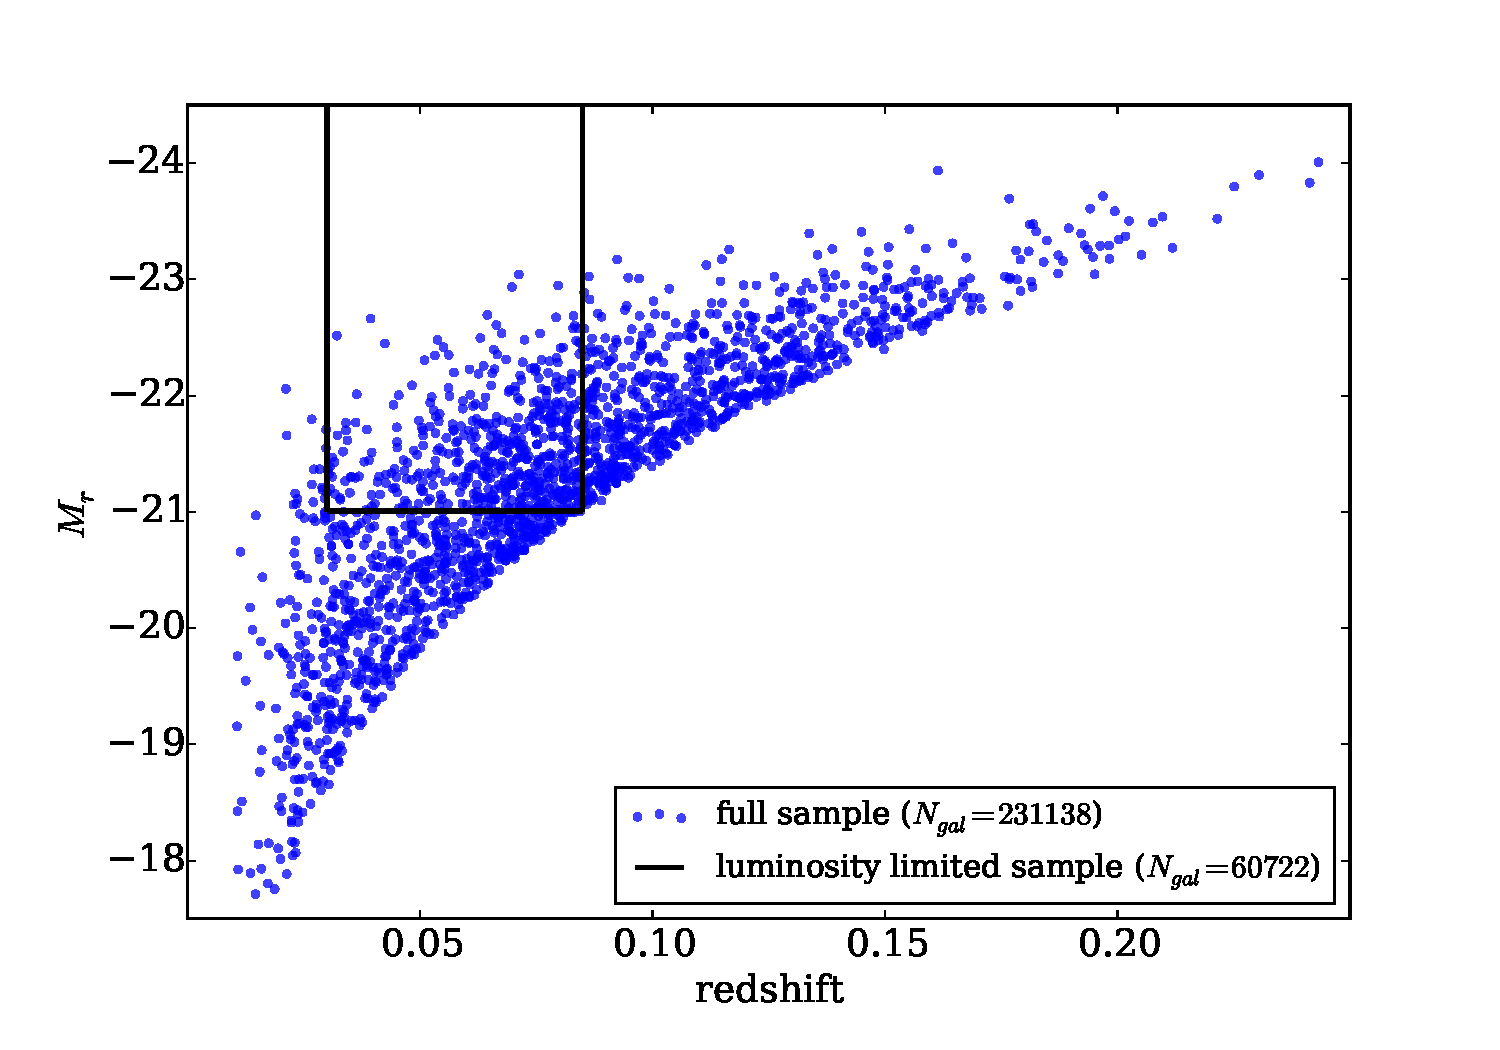
\includegraphics[width=0.5\textwidth]{Data_imgs/volume_limited_sample.pdf}
		
        \caption{Plot indicating the \textit{full sample} (blue points) and the $0.03<z<0.085$ \textit{luminosity limited sample} (region enclosed within the black lines). All galaxies brighter than $M_r  = -21.01$ should be included in the \textit{luminosity limited sample}. A random selection of only 2000 galaxies are plotted for clarity.}
		
        \label{fig:vl_sample}
        
\end{figure}

An upper limit on the redshift that we can use to limit the sample in $M_r$ is imposed at $z=0.085$, as this is redshift to which we have reliable galaxy environmental density data from \cite{Baldry_06}. This was chosen as the redshift limit, as any lower redshift limit would include a smaller number of galaxies. A lower limit of $z_{min}=0.03$ is also imposed to avoid incorrect colour and therefore stellar mass data in nearby galaxies caused by fibre collisions. This gives an absolute magnitude limit of $M_r<-21.01$, and a sample size of 60,722 galaxies. The redshift and absolute magnitude limits imposed to create the \textit{luminosity limited sample} are indicated in figure \ref{fig:vl_sample}. 

Another property that must also be considered for completeness is stellar mass. A relationship between absolute magnitude, colour and stellar mass is observed \citep{Baldry_06}, and the \textit{luminosity limited sample} defined above is incomplete for detecting red galaxies with $\log (M/M_{\odot}) < 10.6$. We therefore consider a further reduced sample of galaxies with $\log (M/M_{\odot}) \geq 10.6$, which is complete for all galaxies brighter than $M_r = -21.01$ and stellar mass $\log (M/M_{\odot}) = 10.6$.  This sample is referred to as the \textit{stellar mass limited sample}.

%------------------------------------------------------------------------------------
%%%%%%%%%%%%%%%%%%%%%%%%%%%%%%%%%%%%%%%%%%%%%%%%%%%%%%%%%%%%%%%%%%%%%%%%%%%%%%%%%%%%%
%------------------------------------------------------------------------------------

\section{Correcting for redshift bias}

\subsection{Different methods for quantifying morphology in Galaxy Zoo}
\label{sec:comaprison_methods}

Galaxy Zoo allows for a statistical analysis of galaxy morphology. Each of the SDSS galaxies has been observed by $\gtrsim 40$ independent classifiers (W13), meaning that galaxy morphology changes can be studied with respect to other properties such as stellar mass, colour or environment. There are two ways in which galaxy morphology can be quantified in Galaxy Zoo. One technique involves looking at the galaxy population as a whole, and looking for any enhancements in vote fractions with respect to a given property \citep{Bamford_09,Casteels_13,Willett_15}\rh{+loads of others}. In this case, the overall Galaxy Zoo vote fractions are used as indicators of morphology within the global galaxy population, with the main advantage being that the sample is not divided in to smaller subsamples, meaning the studied galaxy population remains large.

An alternative method of comparing properties of galaxies with respect to morpholgy would be to divide the galaxy sample in to different morphological categories.  for example, such a method has been used to compare populations of spiral and elliptical galaxies directly \citep{Skibba_09,Smethurst_15} \rh{+loads of others}. It is this type of morphological classification that is the focus of this paper, where spiral arm number is considered. We wish to use this technique because of the relatively low number statistics involved in looking at spiral arm number. Although the overall galaxy population is large in GZ2, with $\sim 60,000$ galaxies in our \textit{luminosity limited sample}, the number statistics are much lower when looking at spiral arm number. This is the case because of the way in which the GZ2 question tree is set up. For a person to classify arm number, they would first have had to have said that the galaxy contained features, was not edge-on and that the galaxy contained spiral structure. The more detailed features, in particular when a galaxy contains 4 or more than 4 spiral arms, can be difficult to discern, meaning that overall vote fractions for such categories is very low. Thus, signals from these galaxies can be very noisy, making it very difficult to observe clear changes in vote fractions as a function of other galaxy properties.

\subsection{Biases in the Galaxy Zoo sample}
\label{sec:biases}
Without any evolution in the population of galaxies, the 'true' distribution of morphologies does not change. However, the apparent brightness and size of galaxies can change depending on the distance at which it is viewed \citep{Bamford_09}. The Galaxy Zoo 2 sample includes SDSS galaxies and only includes galaxies up to a redshift of $\sim 0.25$, which is shallow enough to justify that there is no evolution in the true galaxy morphologies in our sample \citep{Willett_13}. However, the sample is still susceptible to \textit{classification bias}, due to the effect of how the images are presented in Galaxy Zoo. Due to their distance, galaxies at high redshift appear fainter in the SDSS images than galaxies at lower redshift, and therefore have lower signal-to noise. This means that more detailed features may be more difficult to distinguish in galaxies at higher redshift. It should also be noted that such biases are not exclusive to Galaxy Zoo: difficulty in observing faint features in lower signal-to-noise galaxies is an inherent property of visual galaxy classifications. The advantage of using Galaxy Zoo classifications is that it gives us a statistical method of looking at Galaxy morphologies. As each of the galaxies in the full galaxy sample has been visually classified by a number of independent observers, we can model how the apparent presence of features evolves with redshift, and correct this bias accordingly.  \rh{Could maybe include a 'vf vs. z' diagram here to show the apparent evolution in morphology, as per my lunch talk?}

The effect of classification bias is an important property that must be corrected for if we want to compare morphologies using either of the two techniques discussed in section \ref{sec:comaprison_methods}. An biased sample would be affected by defects in two ways. Firstly, samples for the most 'difficult to see' features would be incomplete, meaning that the samples may be affected by poor number statistics. The second issue that would affect the results is sample contamination. This means that subsamples of the 'easier to see' features would actually include several galaxies that have been mis-classified that should have actually be included in the 'harder to see' subsamples. Therefore, any differences in the properties of different sub-samples may be negated due to bias.

\subsubsection{Previous attempt to correct for redshift bias}
\label{sec:previous_method}

\begin{figure}
		\centering
		
        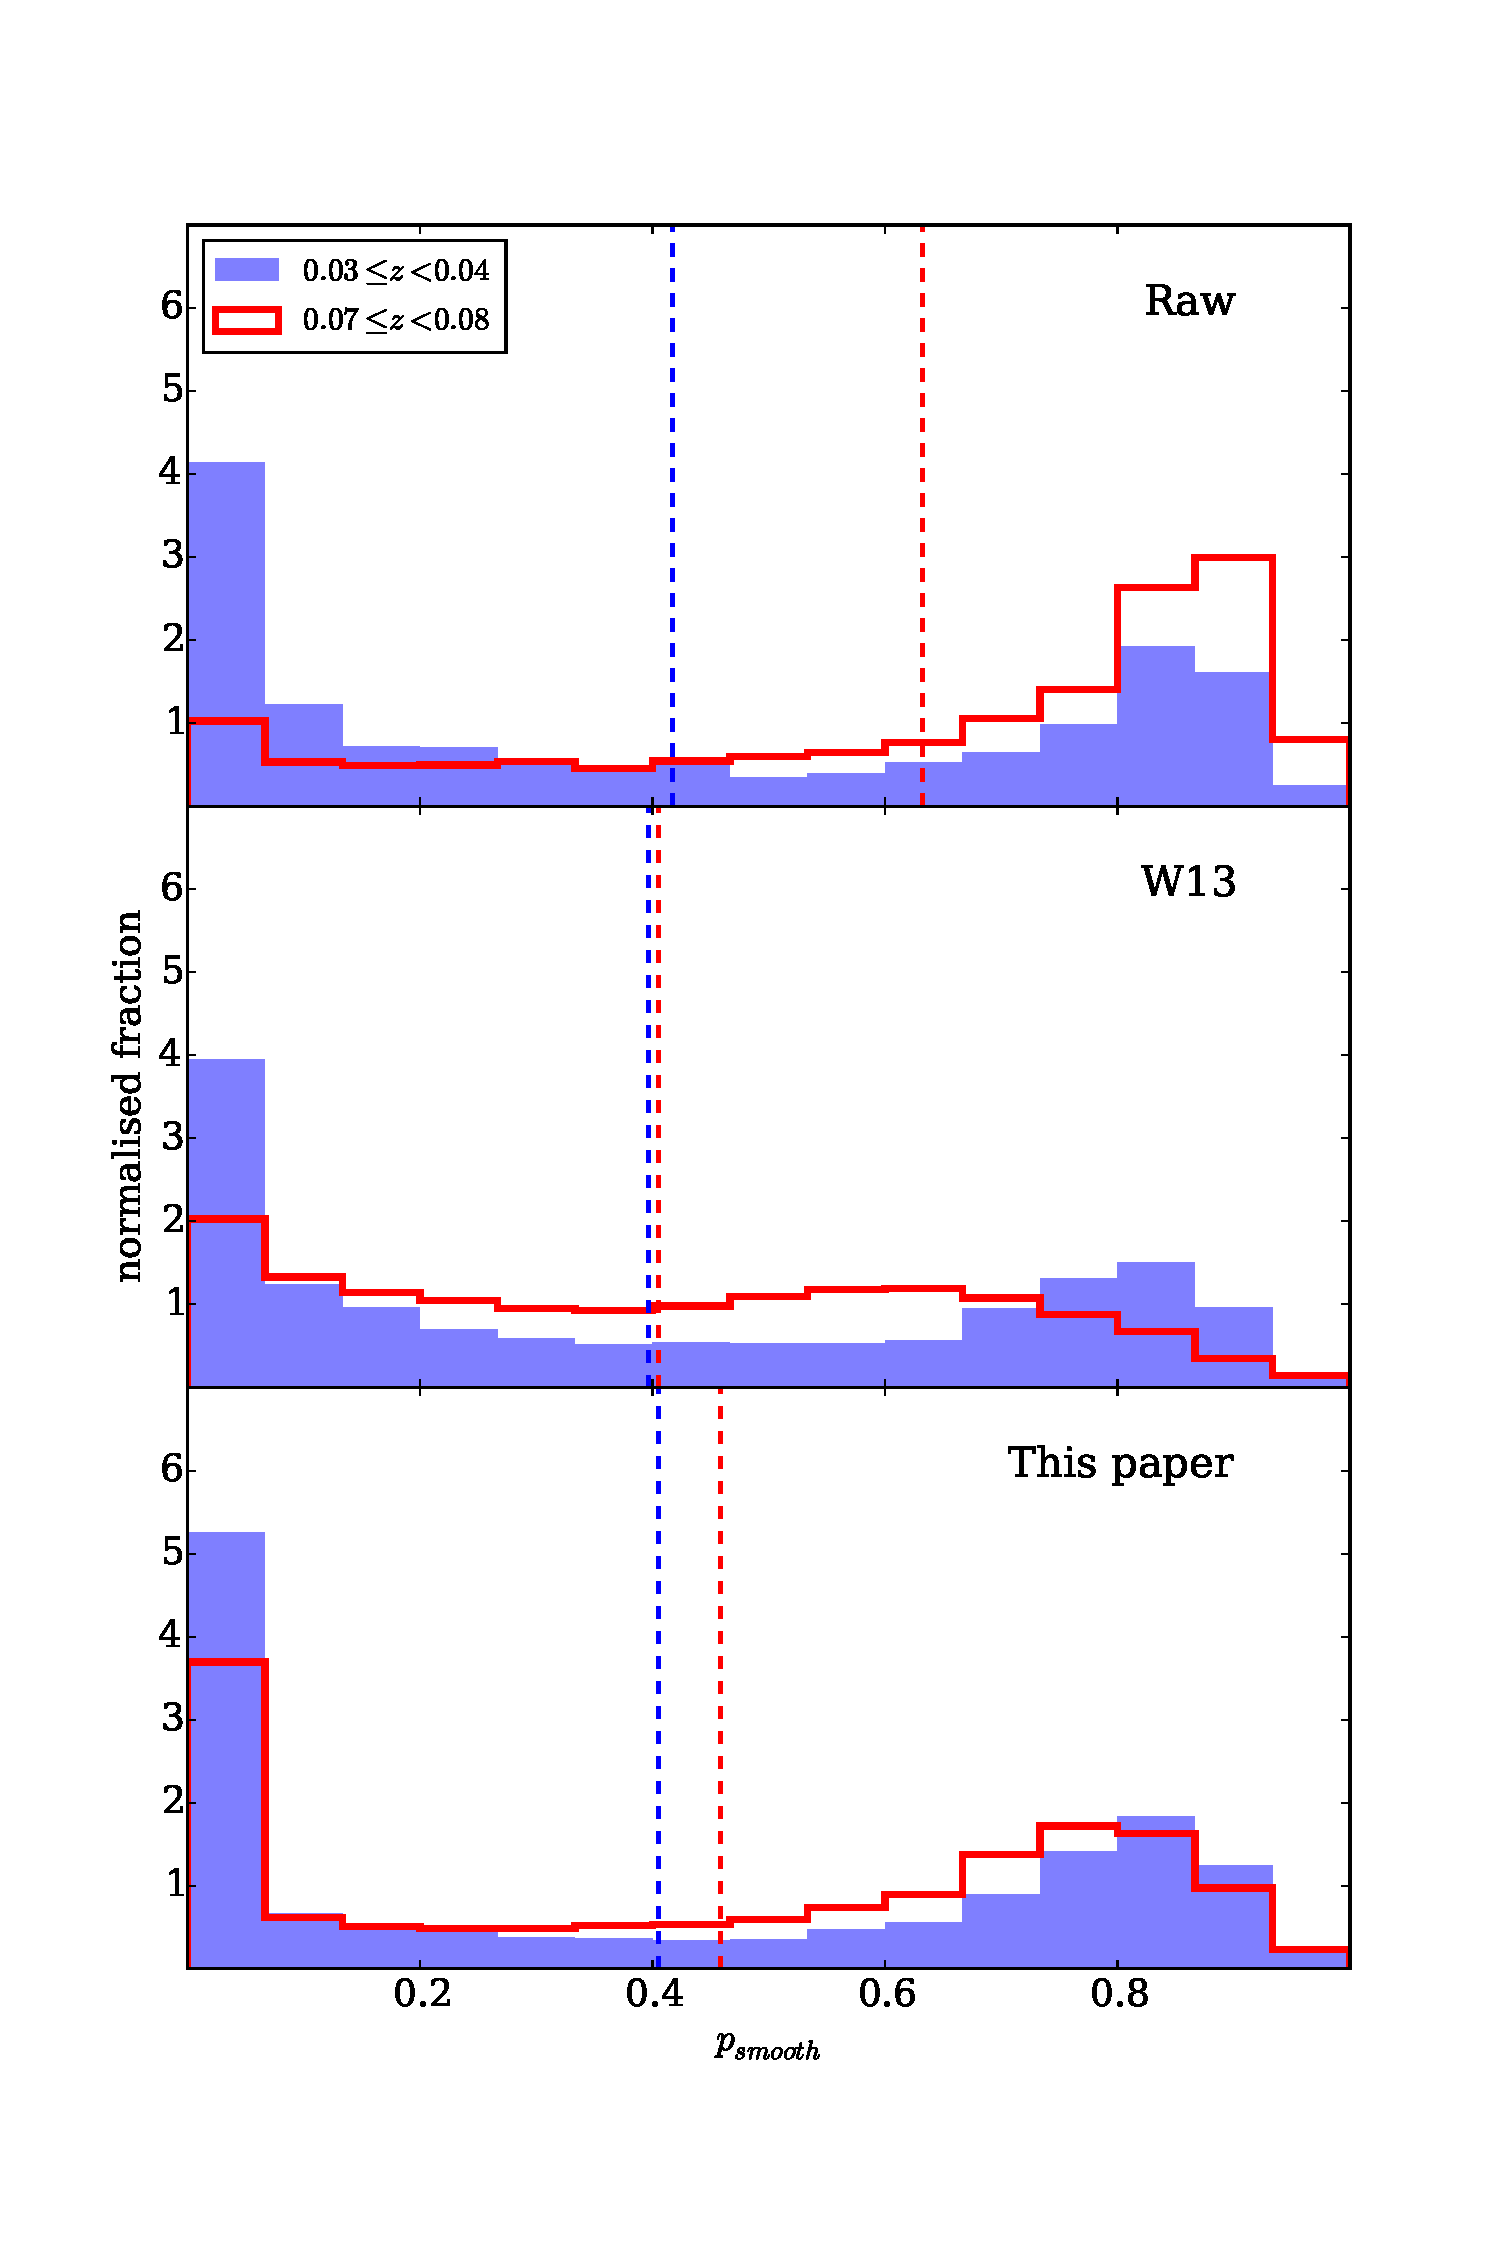
\includegraphics[width=0.5\textwidth]{Data_imgs/vote_distribution_histograms.pdf}
		
        \caption{Histograms of vote distributions for the question of whether galaxies are 'smooth' or contain 'features' in GZ2. The filled blue histogram shows a low redshift sample and the red line indicates a high redshift sample. Both are from the \textit{luminosity limited sample}, so should contain no inherent bias. The dashed blue line indicates the mean from the low redshift sample, and the red dashed line indicates the mean of the high redshift sample.}
		
        \label{fig:vote_histograms}
        
\end{figure}

The previous debiasing procedure applied to both Galaxy Zoo 1 (GZ1) and Galaxy Zoo 2 (GZ2) has focused on adjusting the vote fractions of the galaxy samples by fixing the mean vote fractions as a function of redshift, a method first proposed in \cite{Bamford_09}, and updated for GZ2 in \citep{Willett_13}. However, this technique has two limitations that make it unsuitable if we want to divide a galaxy sample in to different morphology subsets. The first issue is that adjustment of the mean vote fraction does not lead to correct adjustment of individual vote classifications, an effect that can be seen in the middle panel of figure \ref{fig:vote_histograms}. Although the mean fractions for the high redshift sample have been correctly adjusted to match the low redshift sample, the shape of the histogram has not. This means that the number of galaxies that if we wish to define a 'smooth' sample of galaxies from this sample, the number of galaxies that would be correctly classified has a strong dependence on where the vote fraction threshold is made, an effect that is clearly observed in figure \ref{fig:p_bias}. If we were to make a cut at $p_{smooth} > 0.5$, then the sample would be complete. However, if we instead decided to only include galaxies with $p_{smooth} > 0.8$, then the fraction of galaxies that were included with that threshold decreases with redshift, thus making the sample incomplete.

\begin{figure}
		\centering
		
        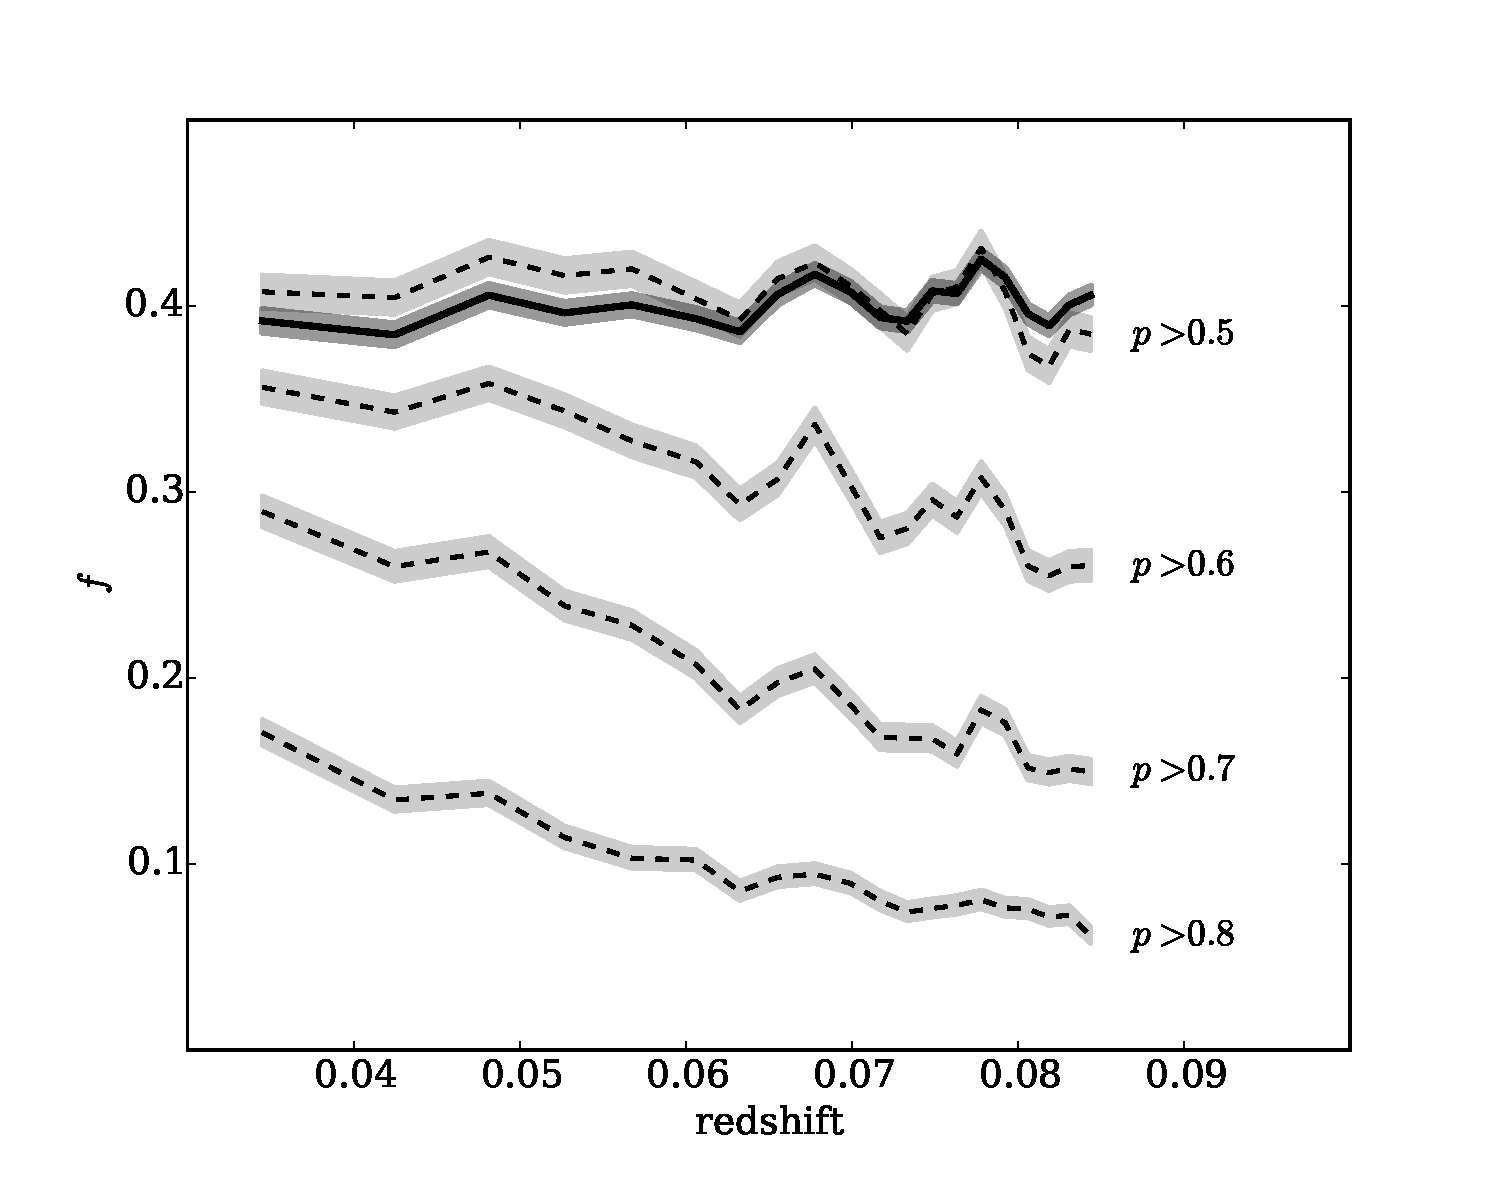
\includegraphics[width=0.5\textwidth]{Data_imgs/p_bias.pdf}
		
        \caption{Fraction of galaxies with $p_{smooth}$ greater than a given threshold as a function of redshift. The solid line indicates the mean value of $p_{sooth}$ as a function of redshift. The dashed lines show the fraction of the total \textit{luminosity limited sample} that meets the $p$ threshold with respect to redshift. The shaded regions indicates the $1 \sigma$ error on the mean for the mean values (solid line) and the $1 \sigma$ fractional errors for each of the $p$ lines, calculated using the method described in \citet{Cameron_11}.}
		
        \label{fig:p_bias}
        
\end{figure}

The second limitation to the debiasing method described in W13 is shown in figure \ref{fig:arm_bias}, where the spiral arm number question of GZ2 is shown. We select a sample of 'secure' spiral galaxies with $p_{features} \times p_{not \, edge-on} \times p_{spiral} > 0.5$, with the $p$ value corresponding to the debiased values from W13. It appears that when considering a question with multiple answers, the debiasing procedure does not do an adequate job in adjusting the mean vote fractions as it does in a question with two main answers, such as 'features or disk'. A clear trend is observed with redshift, where the two armed $\overline{p}$ value increasing with redshift, and the 4 and more than 4 armed $\overline{p}$ values decreasing with redshift. This trend is not effectively removed when considering the debiased values from W13.This would mean that any 2 armed galaxy population that could be selected would be affected by sample contamination from incorrectly classified galaxies. The corresponding 3, 4 and more than 4 armed galaxy populations would suffer from sample incompleteness, leading to poor number statistics. Consequently, to use a thresholding technique to divide our galaxy sample, we require a new debiasing procedure to define our samples to reduce the effects of redshift bias.

\begin{figure}
		\centering
		
        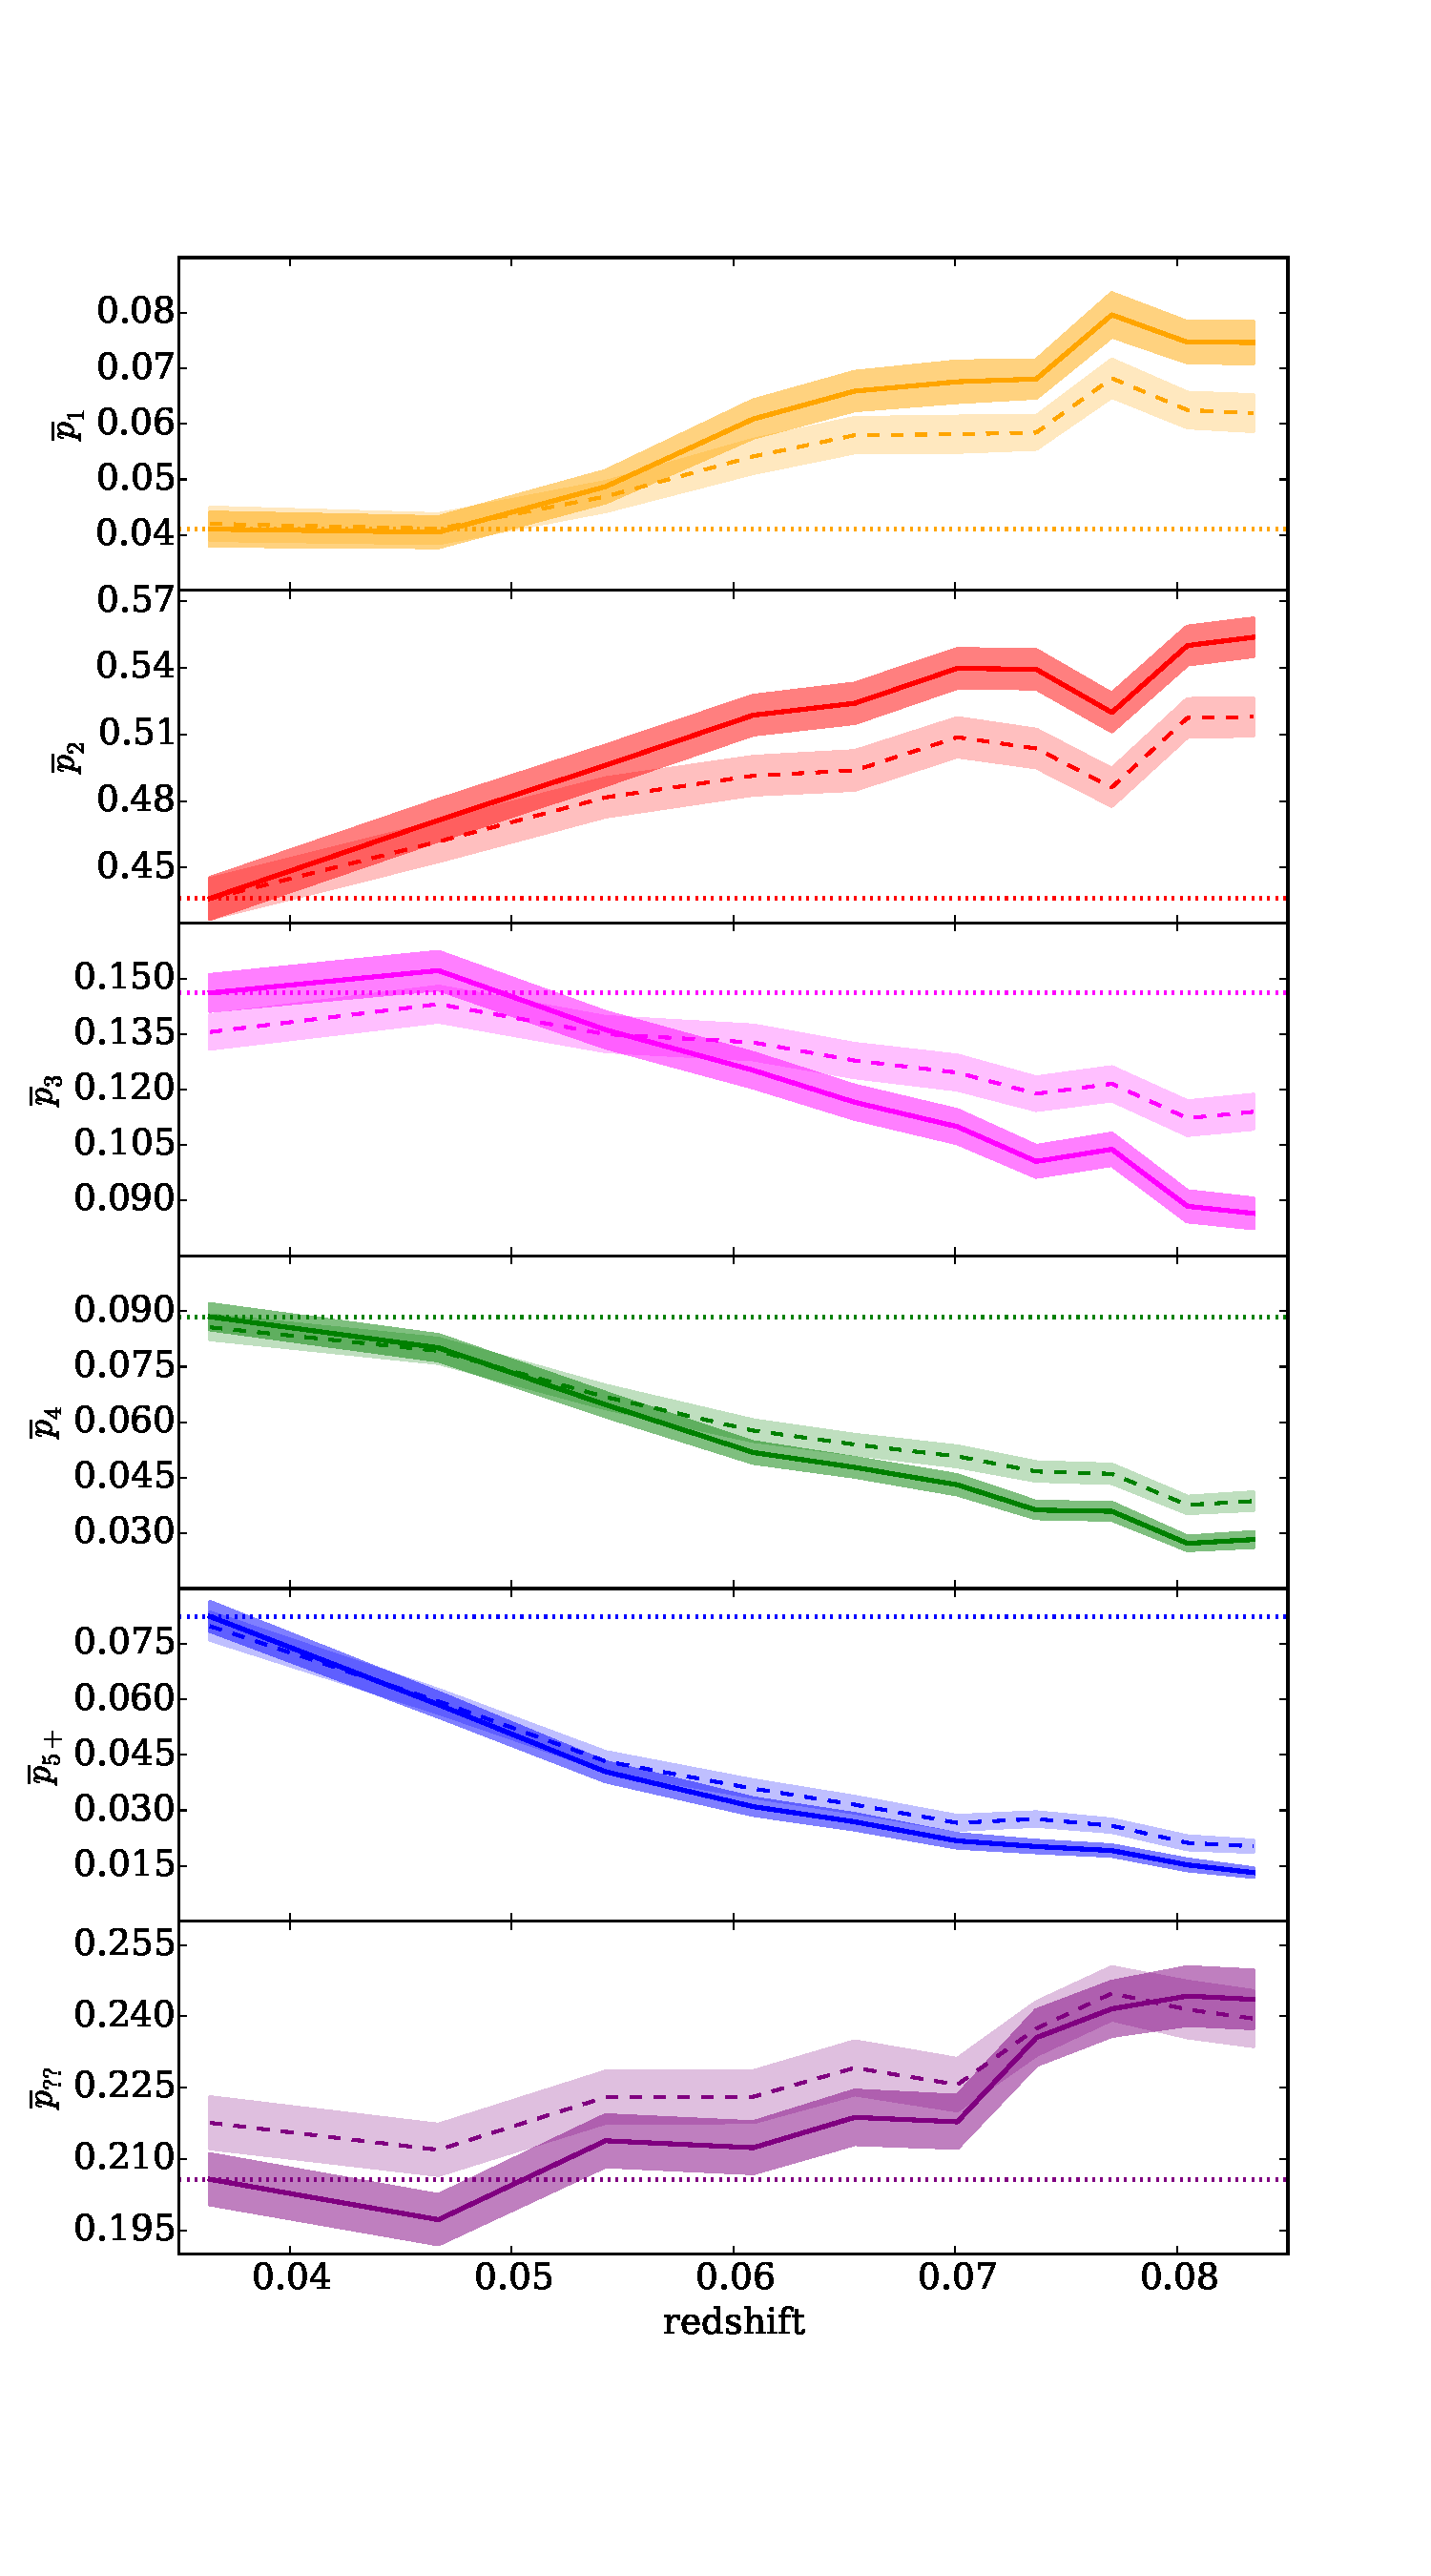
\includegraphics[width=0.5\textwidth]{Data_imgs/arm_bias.pdf}
		
        \caption{Mean value of $p$ for each of the arm numbers in the \textit{luminosity limited sample}. The shaded regions indicates the $1 \sigma$ error on the mean. The solid lines show the values obtained using the raw vote classifications, and the dashed lines indicate the corresponding values from the debiased values from W13. The dotted lines indicate the $p$ value from the low redshift bin for reference.}
		
        \label{fig:arm_bias}
        
\end{figure}

\subsection{A new method for removing redshift bias}
\label{sec:new_method}

With the limitations described in section \ref{sec:previous_method}, we attempt to construct a new method of debiasing the GZ2 data more effectively. The new method aims to make the vote distributions themselves as consistent  as possible with redshift rather than aiming for consistency in the mean vote fraction values. This debiasing method is made possible due to the number of individual classifications we have of each of the galaxies in our sample. As each galaxy is classified by 40 or more volunteers (W13), we have enough data to model the evolution of the vote fractions as a function of redshift. The main motivation behind this method is that different classifiers will have different levels of ability to pick out the most detailed features. Thus, as we consider samples at higher redshift, where images have lower signal-to noise, we expect the overall vote fraction trend to also evolve as some classifiers become less able to see the most detailed features. We aim to model this redshift bias by modelling the vote fraction histograms as a function of redshift, and correcting the higher redshift vote distributions to be as similar as possible to equivalent vote distributions at low redshift.

\subsubsection{Sample selection for each question}

As GZ2 morphologies are classified with a decision tree (described in more detail in W13), not all of the questions were answered by each of the volunteers. Using the example of spiral arm number, for an individual classifier to have answered the question regarding arm number, they would also have needed to answer that the galaxy they saw had features, was not edge-on and had spiral arms. To avoid 'noise' introduced by incorrectly classified galaxies, clean galaxy samples are defined with $p > 0.5$. For the first question, this corresponds to all of the galaxies, as each classifier answered that particular question for each galaxy. However, when questions further down the tree are considered, this is not the case. The equiavalent $p>0.5$ for the spiral arm question for example would therefore only include the galaxies with $p_{features} \times p_{not \, edge-on} \times p_{spiral} > 0.5$. A cut of $N \geq 0.5$ is also imposed to ensure that each galaxy has been looked at by a significant number of people to redsuce the effects of noise. In this case, the $p$ values are the debiased vote values, to ensure each sample is as complete as possible (see section \ref{sec:biases}). This also means that the order in which each of the questions is debiased must be taken in to account- each of the questions can only be debiased if questions 'further up' the tree have already been debiased. 

\begin{figure}
		\centering
		
        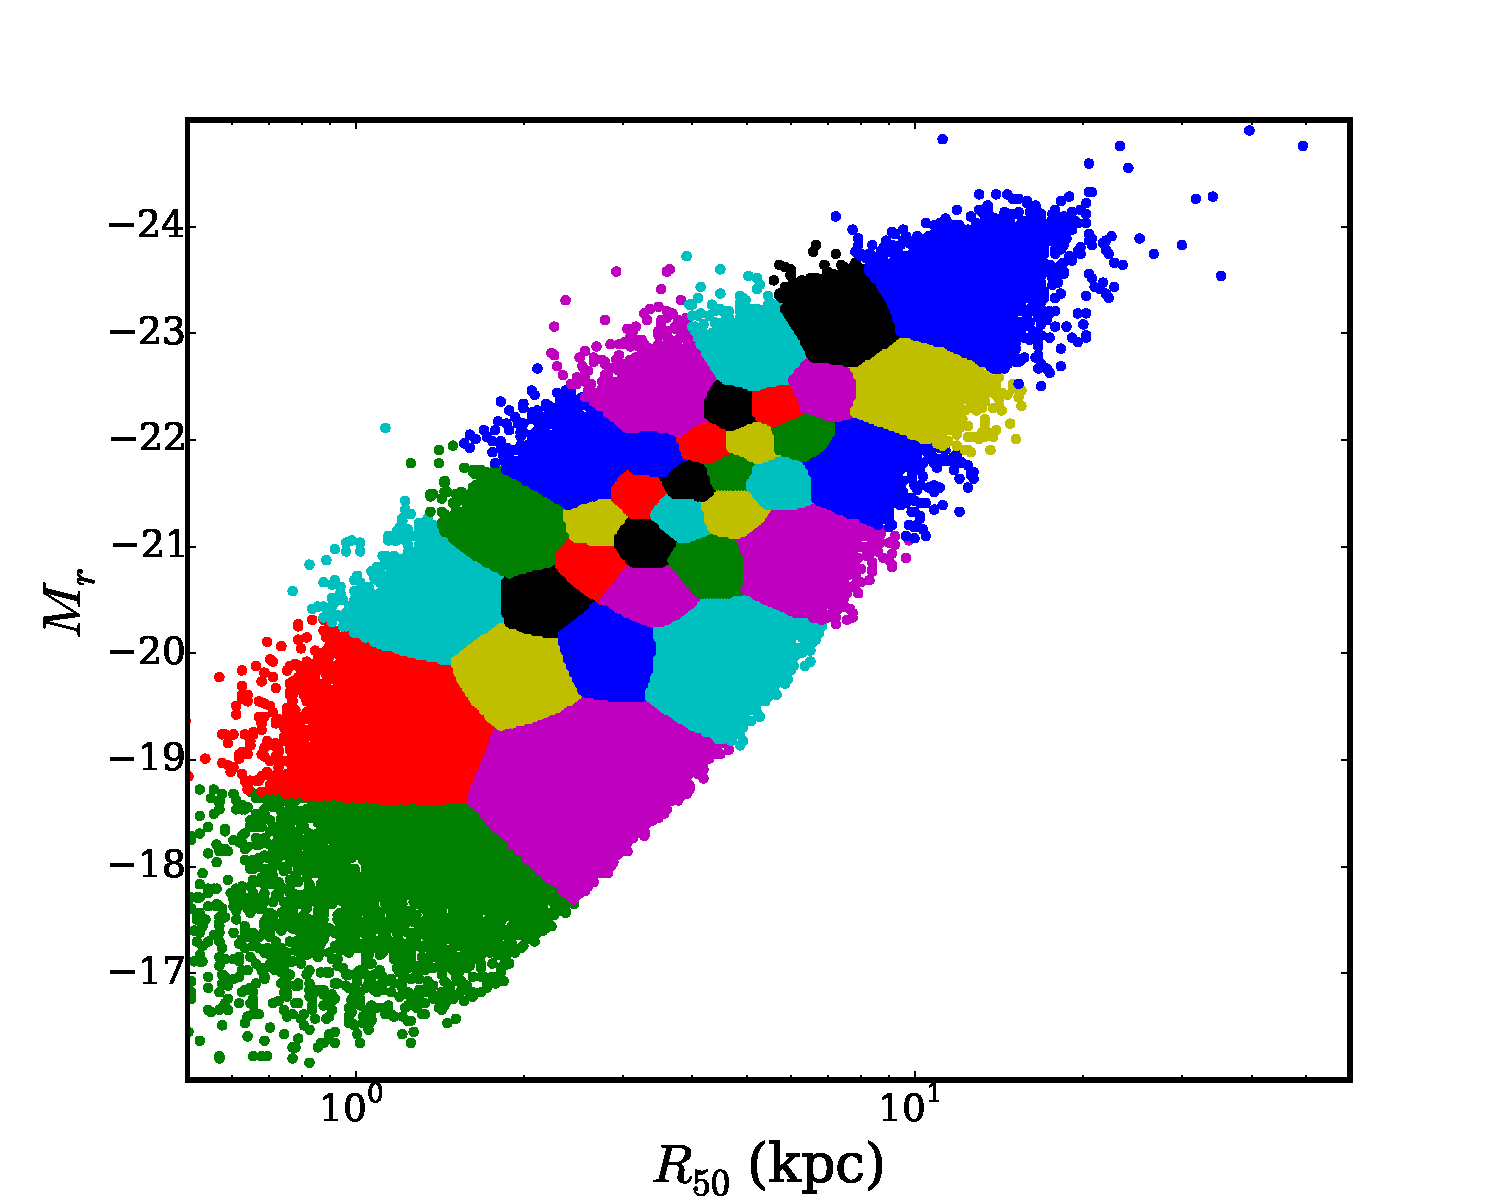
\includegraphics[width=0.5\textwidth]{Bias_imgs/voronoi_bins.pdf}
		
        \caption{Distribution of the voronoi bins in terms of $R_{50}$ and $M_r$. The bins were calculated using the method described in \rh{cite?}.} 
		
        \label{fig:voronoi_bins}
        
\end{figure}

\subsubsection{Binning the data}

To attempt to maximise our signal (the number of galaxies in each bin), we remove any galaxies with vote fractions for a given answer with a value of $p=0$, as these galaxies will not contribute to the 'signal' in each of the bins. It is imperative that intrinsic galaxy properties are accounted for, as there is expected to be an evolution in galaxy properties with different sizes and luminosities \rh{cite?}. To even out the 'signal' and 'noise' in each of the bins, we voronoi tesselate in terms of $M_r$ and $R_{50}$ for each answer in turn, meaning that each of the bins should contain an equal number of galaxies with $p>0$. We aim to have $\sim 30$ voronoi bins for each of the questions, so the bin signal is given as $N/30$, where $N$ is the number of galaxies with $p>0$. Each of these voronoi bins is then further divided in to 5 redshift bins, to allow for the modelling of the vote distributions with respect to redshift, $z$. Thus, for each of the answers, the data is divided up in to approximately equal bins of $M_r$, $R_{50}$ and $z$, to allow us to model the change in vote fraction in terms of both intrinsic galaxy properties (surface brightness) and apparent bias with redshift (described in section \ref{sec:biases}). An example of the voronoi binning is shown in figure \ref{fig:voronoi_bins}.

\subsubsection{Modelling redshift bias}

Having divided the sample in to different bins to allow us to model for intrinsic galaxy properties, we can now attempt to correct for the apparent evolution induced by classification bias as a function of redshift. After dividing the sample in to different redshift bins for each of the voronoi bins, we now fit functions to model the data in each of the bins. To do this, we model the data in terms of $\log(f_v)$, where $f_v$ is the vote fraction for a given question vs. the cumulative fraction. Modelling the cumulative histograms in $\log$ space effectively stretches out the histogram at the lowest end ($f_v \approx 0$). This is particularly useful for the questions where the vote fractions are split between multiple categories, such as the question about the number of spiral arms, as most of the votes are concentrated at $f_v \approx 0$. For each of the redshift bins in turn, and each of the voronoi bins in turn, a cumulative histogram is plotted and a function is fit to model the shape of that particular histogram. We attempt to model each of the histograms with a function describing its overall behaviour. Two functions are used to model the data. The functions selected are a logistic function and an exponential power function, and their equations are listed below:

\begin{center}
$f(x) = \frac{L}{1+e^{-k(x-c)}}$
\end{center}

\begin{center}
$f(x) = e^{kx^{c}}$
\end{center}

where k and c parameterise the shape of each of the curves. We fix the $L$ term with respect to $c$ in the logistic function so that any curve passes through the point $(0,1)$, corresponding to a cumulative fraction of $1$ when $f_v = 1$.All of the functions pass through $(-\infty,0)$ and $(0,1)$, meaning that there is a single cumulative fraction that corresponds to each of the possible values of $0 \leq f_v \leq 1$. A single function is chosen to fit to all of the individual answers, by fitting each of the functions to the total data for each answer, and selecting the function which has the lowest $\chi^2$ value as calculated using the Python $scipy.optimize.minimize$ package. 

After selecting a function, a function is fit to each of the bins calculating optimal $k$ and $c$ values. After calculating a $k$ and $c$ value for each of the bins, a linear function is applied to parameterise how $k$ and $c$ vary with $R_{50}$, $M_r$ and $z$, by fitting a linear function of the following form:

\begin{center}
$k = k_1M_r + k_2R_{50} +k_3z + k_4$
\end{center}

where $k_1$,$k_2$,$k_3$ parameterise the change in $k$ or $c$ with respect to $M_r$, $R_{50}$ and $z$ respectively and $k_4$ is a constant. The $k$ value corresponds to the $k$ or $c$ value that parameterises the curve's shape. the same method is applied to model the second value, $c$ independently. We use these calculated $k$ and $c$ values to estimate the shape of the cumulative histogram function for each galaxy with respect to its $R_{50}$, $M_r$ and $z$. We then use the same linear fits  correct the estimated histogram shape to its equivalent function with $z=0.03$, the lower redshift limit of the data. An example of the curves fit to the arm number answers is shown in figure \ref{fig:function_fit}. 

\begin{figure}
		\centering
		
        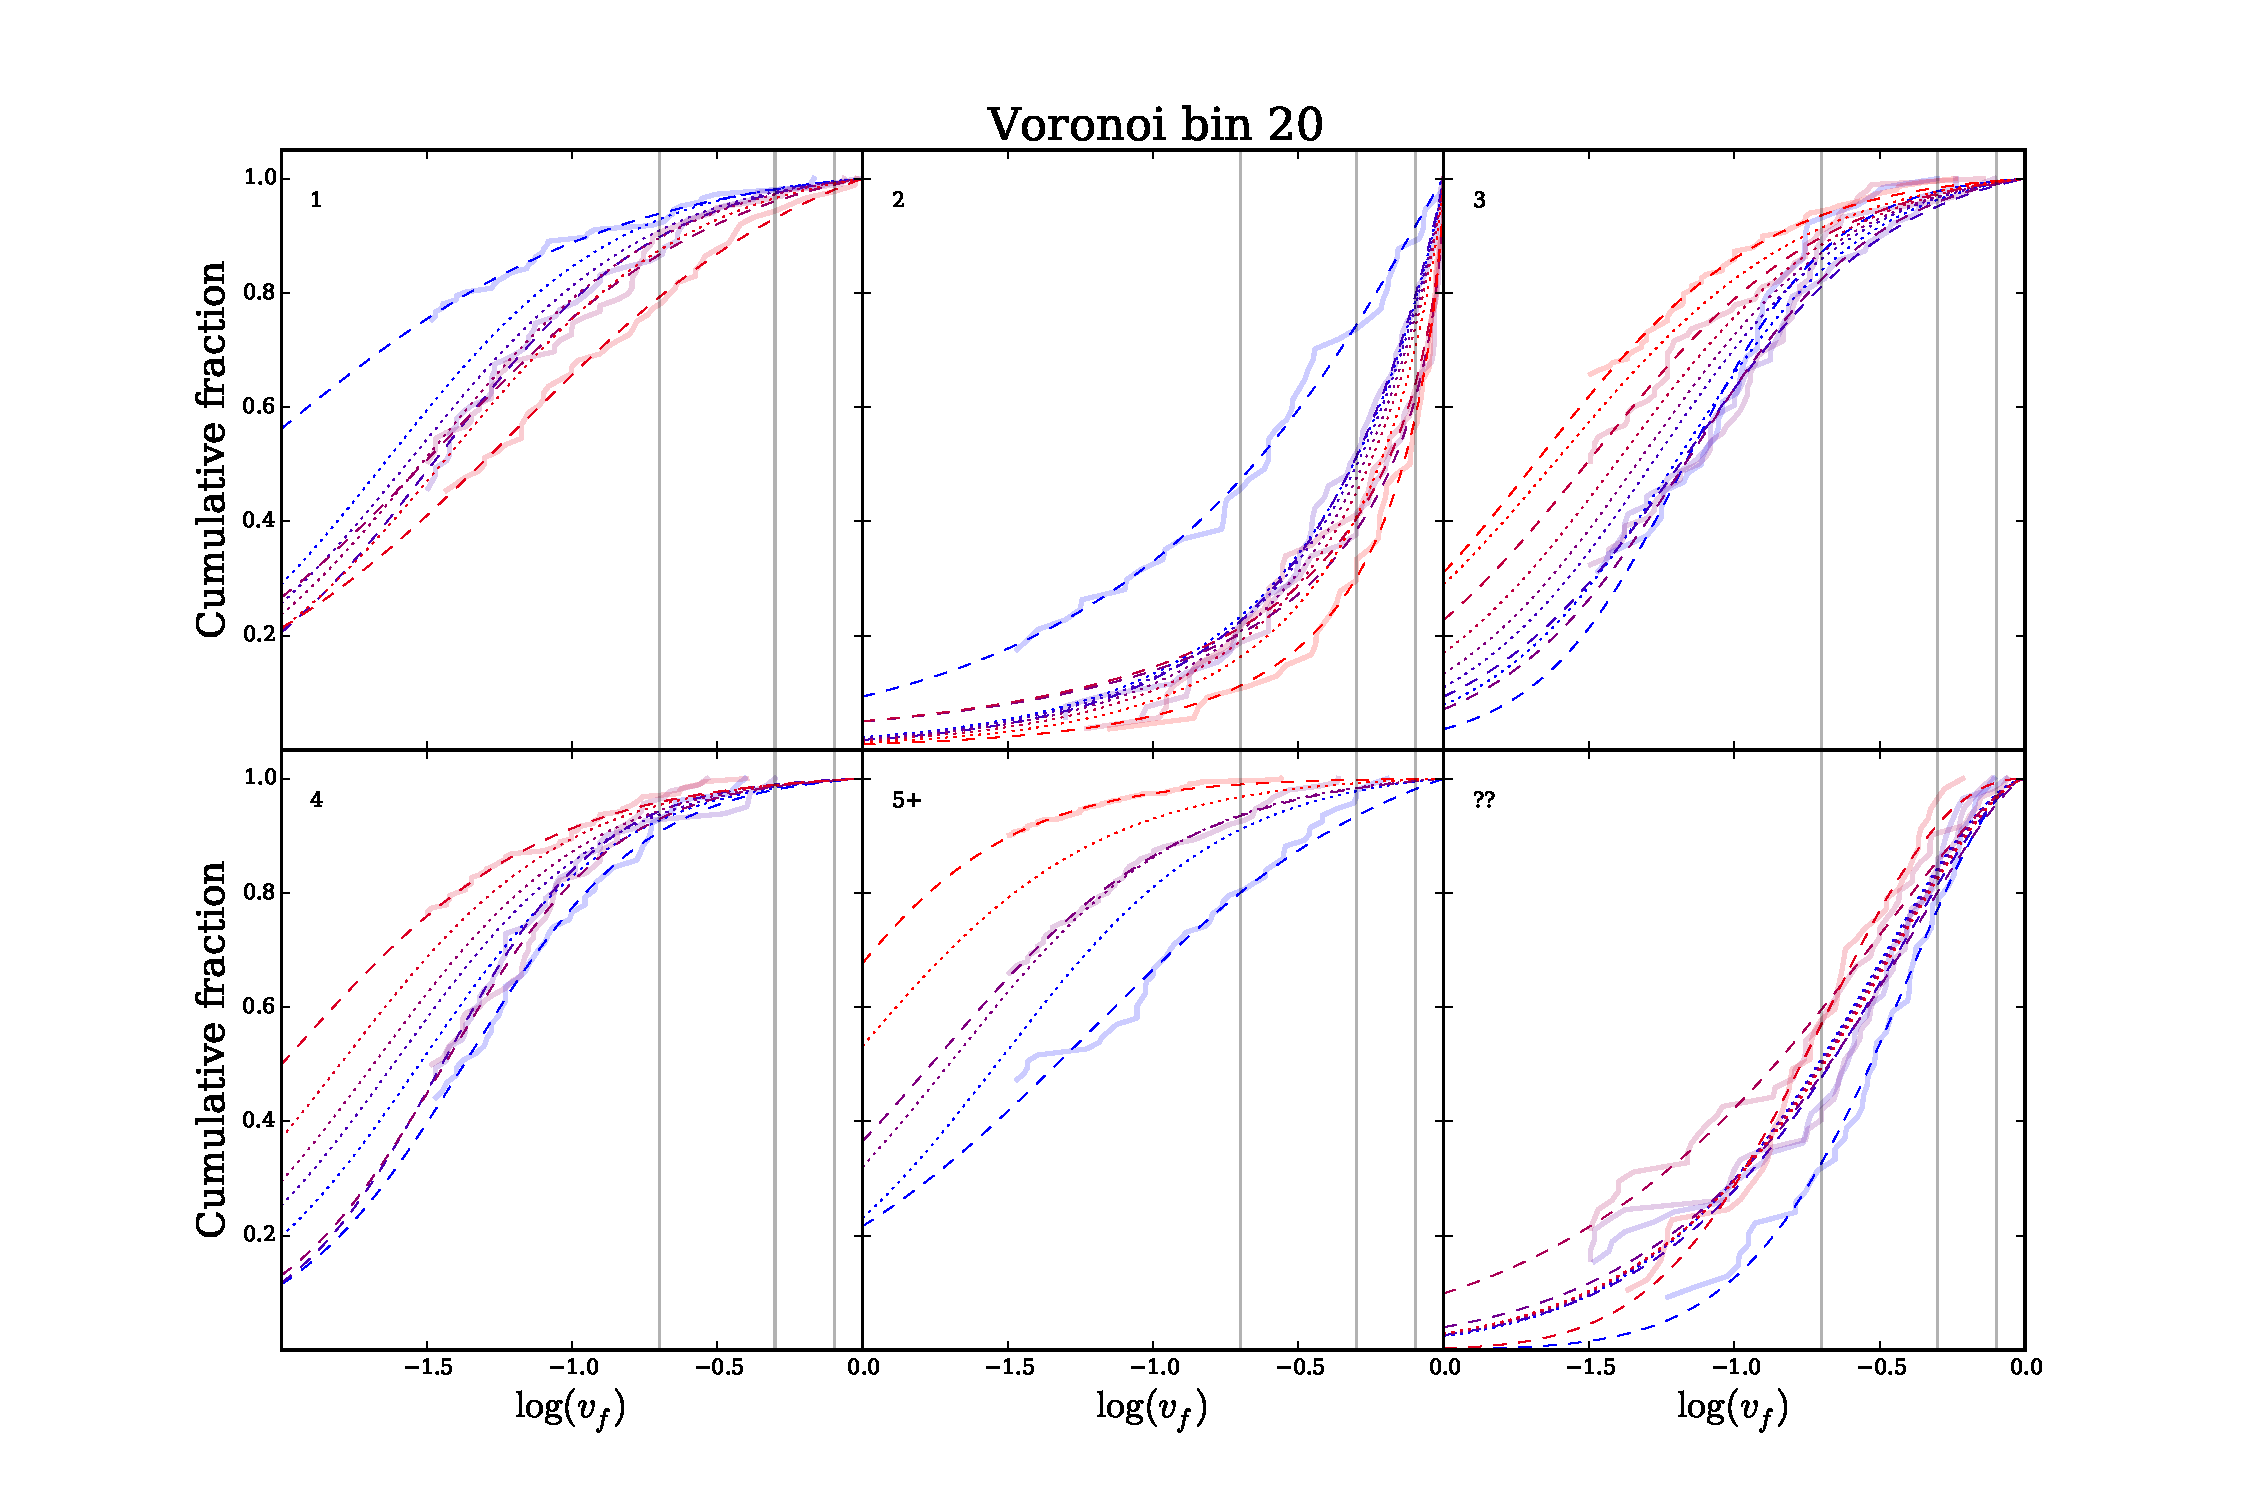
\includegraphics[width=0.5\textwidth]{Data_imgs/fit_t11_arms_number_vbin20_kcfit1.pdf}
		
        \caption{An example of a single voronoi bin fit for arm number. The red line indicates the highest redshift bin, and the blue line indicates the lowest redshift bin. The solid lines indicate the raw $f_v$ histograms, and the dashed lines show the best fit function to each of the corresponding histograms. The dotted lines show the corresponding approximation from the linear fit to the $k$ and $c$ values.}
		
        \label{fig:function_fit}
        
\end{figure}

\subsubsection{Results from the new debiasing method}

\begin{figure*}
		\centering
		
        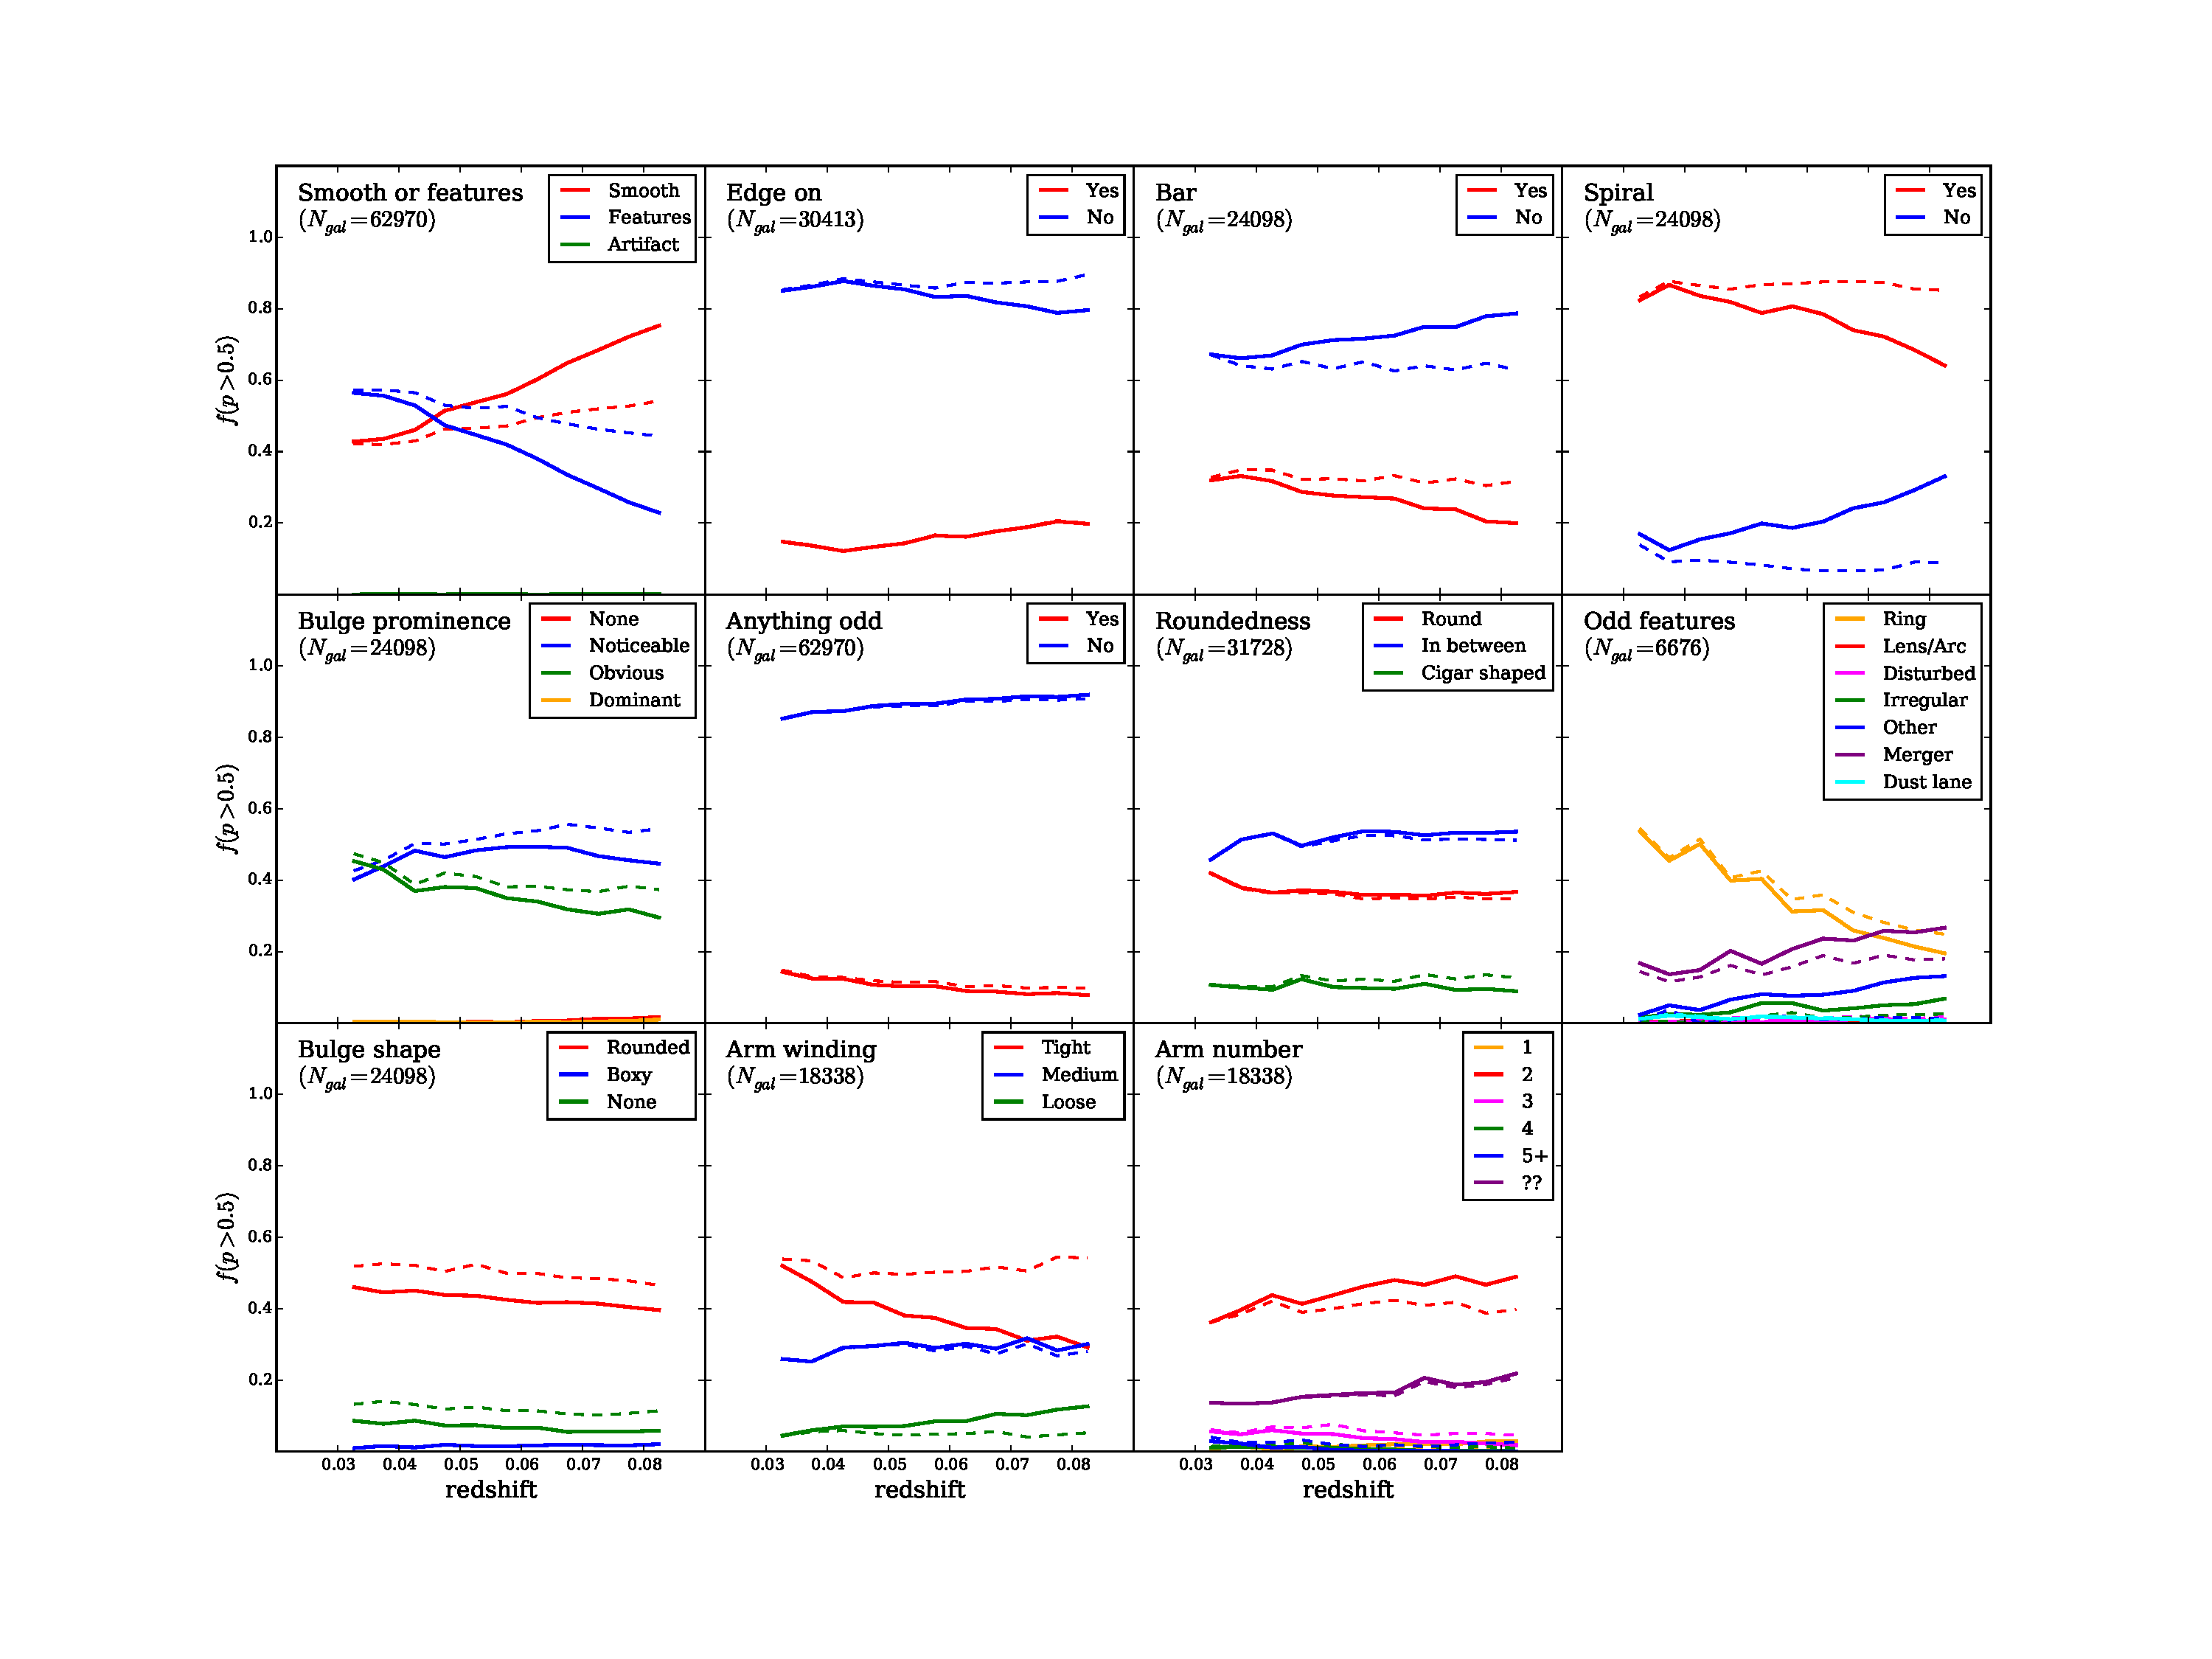
\includegraphics[width=1\textwidth]{Bias_imgs/vote_panel_plot_debiased.pdf}
		
        \caption{Number of galaxies with $p>0.5$ for each of the questions debiased using the method described in section \ref{sec:new_method}. The solid lines indicate the raw vote fractions and the dashed lines indicate the debiased vote fractions. Each of the samples is composed of galaxies with $p_{debiased}>0.5$ of people having answered that particular question.}
		
        \label{fig:vote_panel_debiased}
        
\end{figure*}

Figure \ref{fig:vote_panel_debiased} shows the vote fractions as a function of redshift for the \textit{luminosity limited sample}. Such a sample should be spectroscopically complete at all redshifts, so we expect to see no evolution in galaxy properties with redshift in such a sample. Each of the samples is defined in the same way as described in section \ref{sec:previous_method}. The figures show that when we define samples by making selection cuts at $p>0.5$, the new debiasing procedure removes the apparent redshift evolution more consistently than the previous method employed in \citet{Willett_13}. In particular, we see that if we wish to define a spiral sample imposing a cut of $p_{features} \times p_{not \, edge \, on} \times p_{spiral} > 0.5$, to look in to spiral arm number, then the sample is more complete. It appears that the previous debiasing procedure did not debias the 'spiral' question effectively, leading to incomplete samples of spiral galaxies at higher redshift. In our debiasing procedure, we effectively 'flatten out' the fraction of galaxies with $p_spiral>0.5$ with redshift, as can be seen from the top right hand panel of figure \ref{fig:vote_panel_debiased}. 

%------------------------------------------------------------------------------------
%%%%%%%%%%%%%%%%%%%%%%%%%%%%%%%%%%%%%%%%%%%%%%%%%%%%%%%%%%%%%%%%%%%%%%%%%%%%%%%%%%%%%
%------------------------------------------------------------------------------------
\section{Application to arm number}
\label{sec:results}

%------------------------------------------------------------------------------------

\subsection{Defining the sample}

\rh{Put table here}

\begin{figure}
		\centering
		
        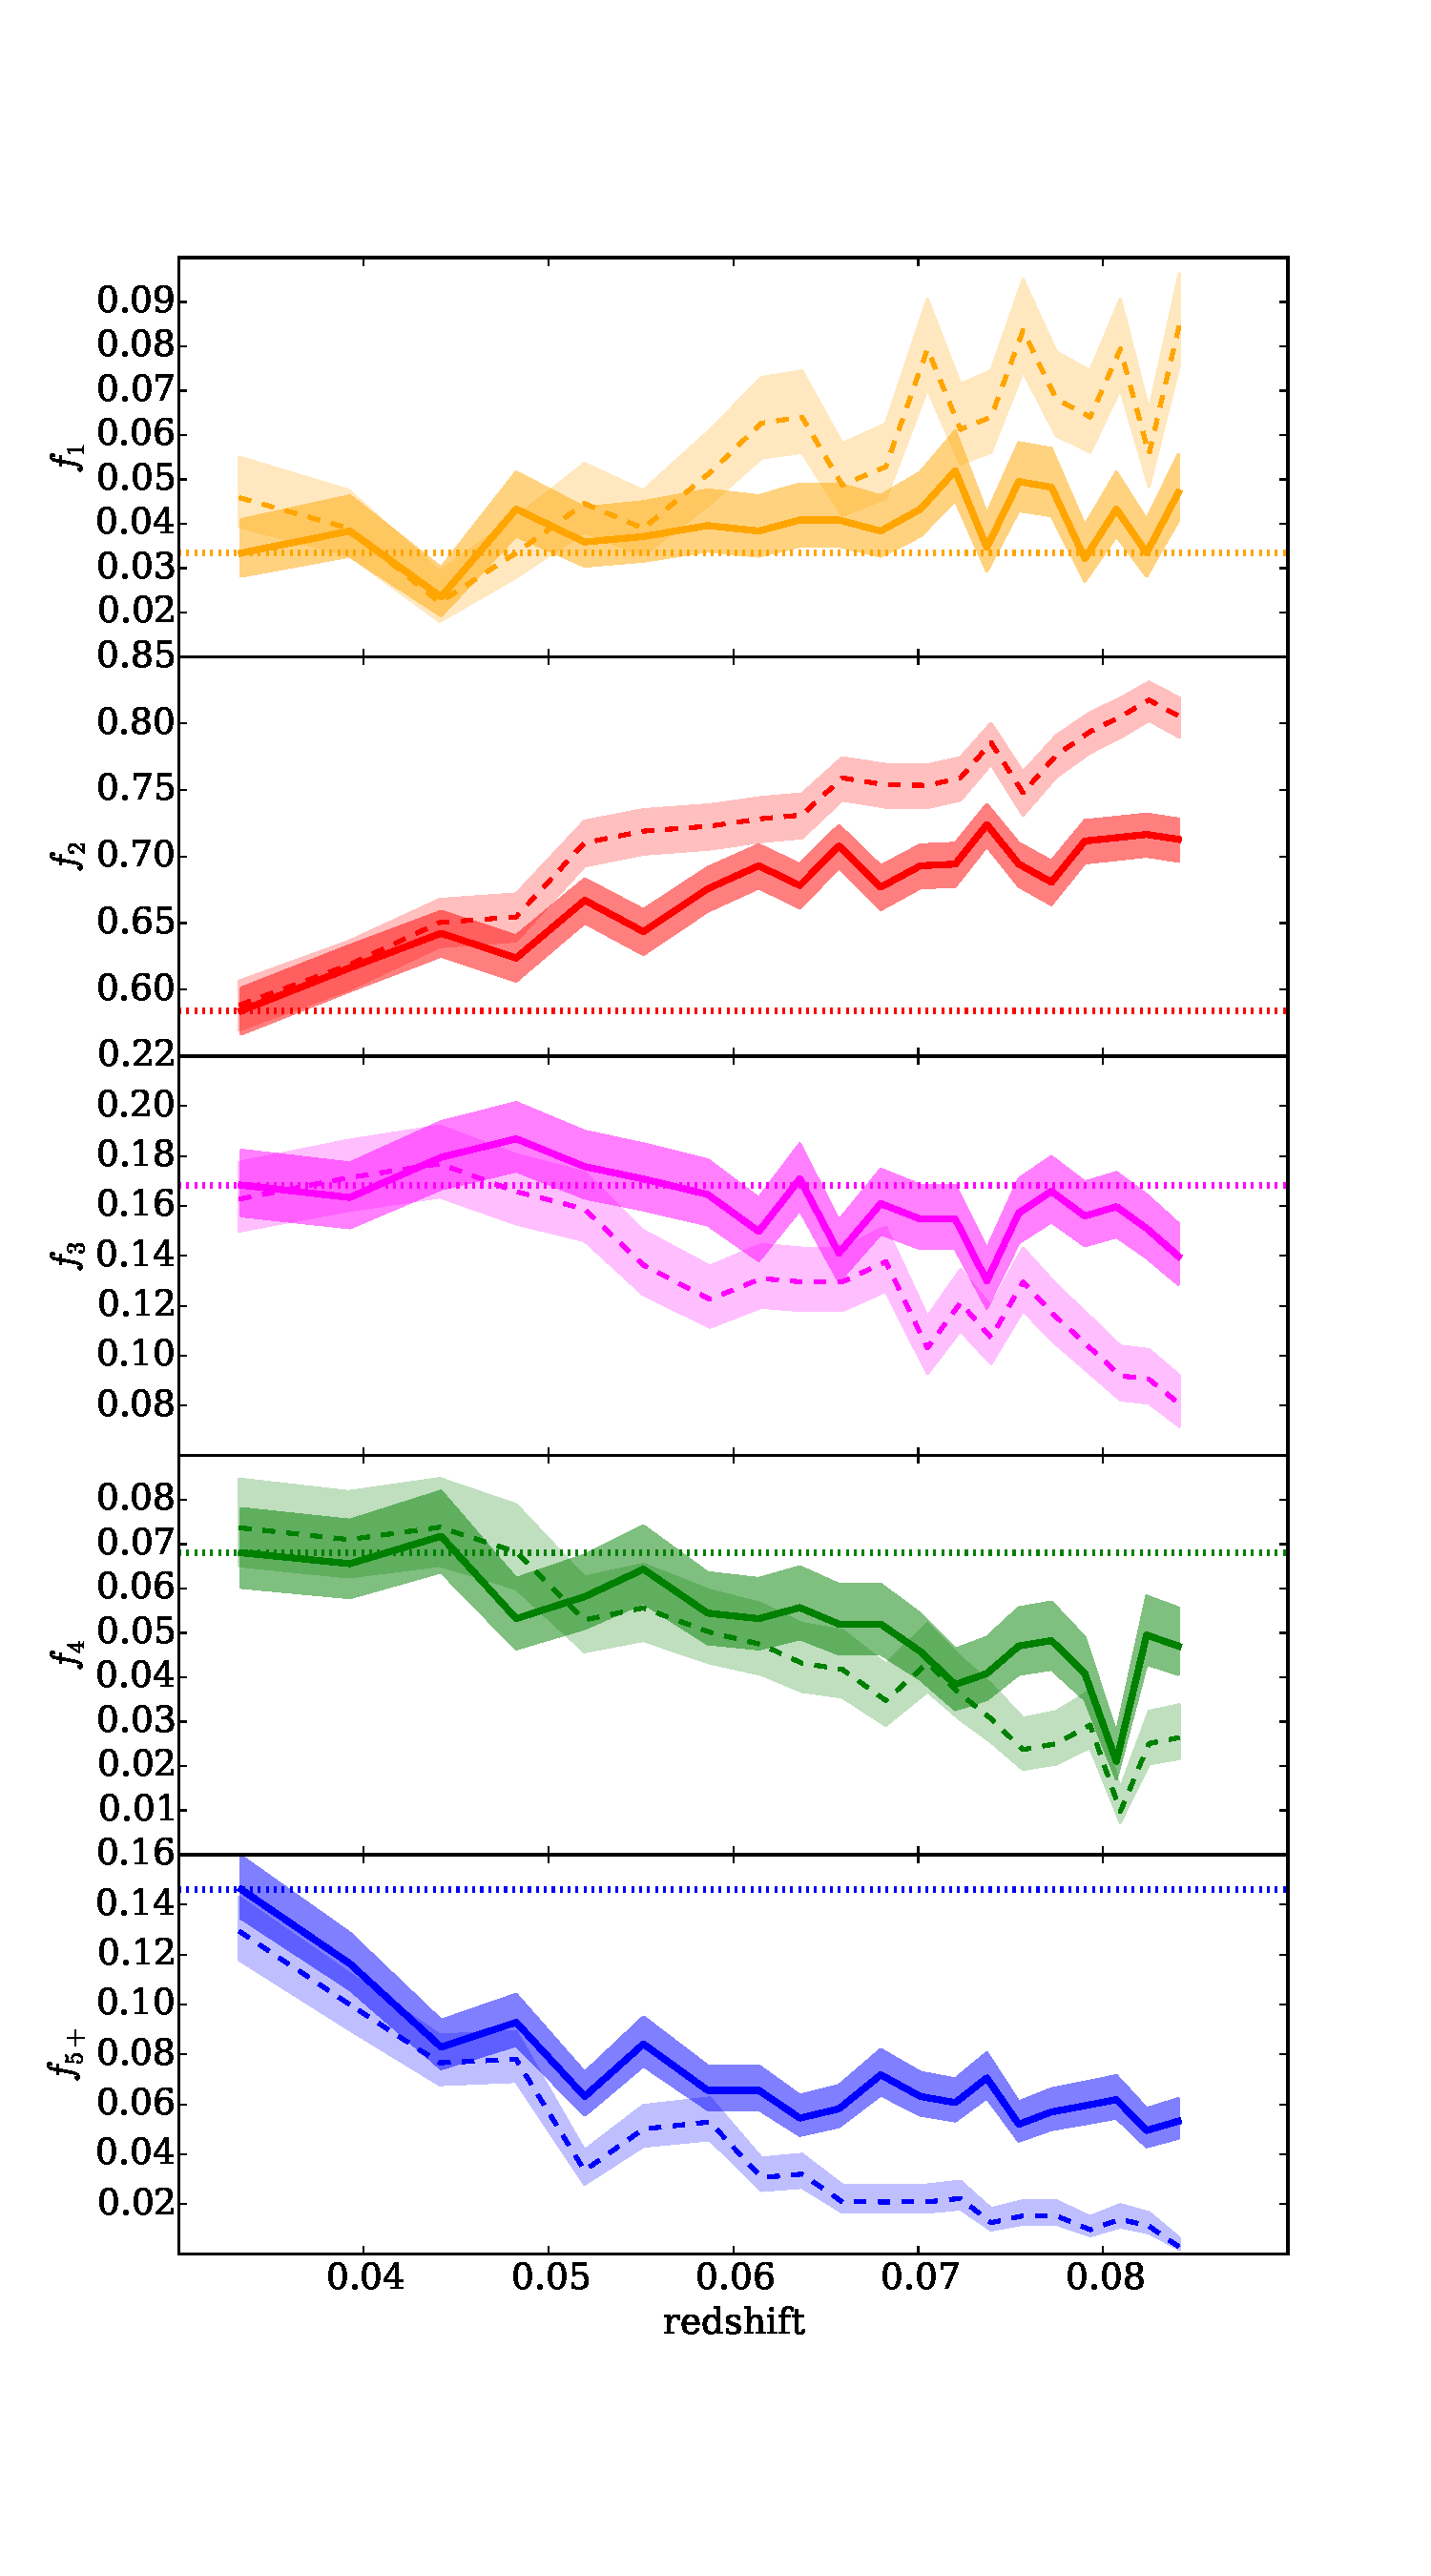
\includegraphics[width=0.5\textwidth]{Data_imgs/redshift_plot.pdf}
		
        \caption{Fraction of galaxies in the \textit{luminosity limited sample} classified as having 1,2,3,4, or more than 4 spiral arms as a function of redshift. The solid line indicates the debiased fractions, and the dashed line indicates the raw vote fractions. Errors are calculated using the method described in \citet{Cameron_11}. The dotted lines indicate the corresponding fraction in the lowest redshift bin for reference.}
		
        \label{fig:arm_number_trend}
        
\end{figure}

An interesting question that has not been fully unexplored in GZ2 is the question of spiral arm multiplicity, or how many spiral arms galaxies have. The star forming properties have already been looked at using the vote fractions \citep{Willett_15}, but we wish to separate the galaxies in to separate populations to compare their properties.The new debiasing method is used to define a sample of galaxies that are classified as spiral galaxies with $p_{features} \times p_{not \, edge \, on} \times p_{spiral} > 0.5$. We also impose the cut of $N>5$, so that each of the galaxies has been observed by more than 5 people to make our selection less sensitive to noise. As a reference, samples selected in the same way using the original debiasing in \citet{Willett_13} are compared. Galaxies are assigned to the spiral arm number by the highest value from the six possible answers to the spiral arm question. However, to maximise our galaxy samples, we also redistribute galaxies that have the highest debiased vote fraction for the 'can't tell' answer. The only limit that is applied is that we still include $N>5$ limit, but this time ignoring the 'can't tells'. All galaxies assigned as spirals in the \textit{luminosity limited sample} that have $>5$ individual classifications of arm number therefore make up our spiral sample. The fraction of galaxies with different arm numbers with respect to redshift are displayed in figure \ref{fig:arm_number_trend} and the overall properties of each of the populations are shown in table XX below. It can be seen from figure \ref{fig:arm_number_trend} that the new debiasing method means that samples are more complete in the higher redshift images. Figure \ref{fig:image_panel} shows a set of images at different redshifts classified as having either 1, 2, 3, 4 or more than 4 arms in different redshift bins. The basic properties of the galaxies in the spiral galaxy sample divided by spiral arm number are compared below.

\begin{figure*}
		\centering
		
        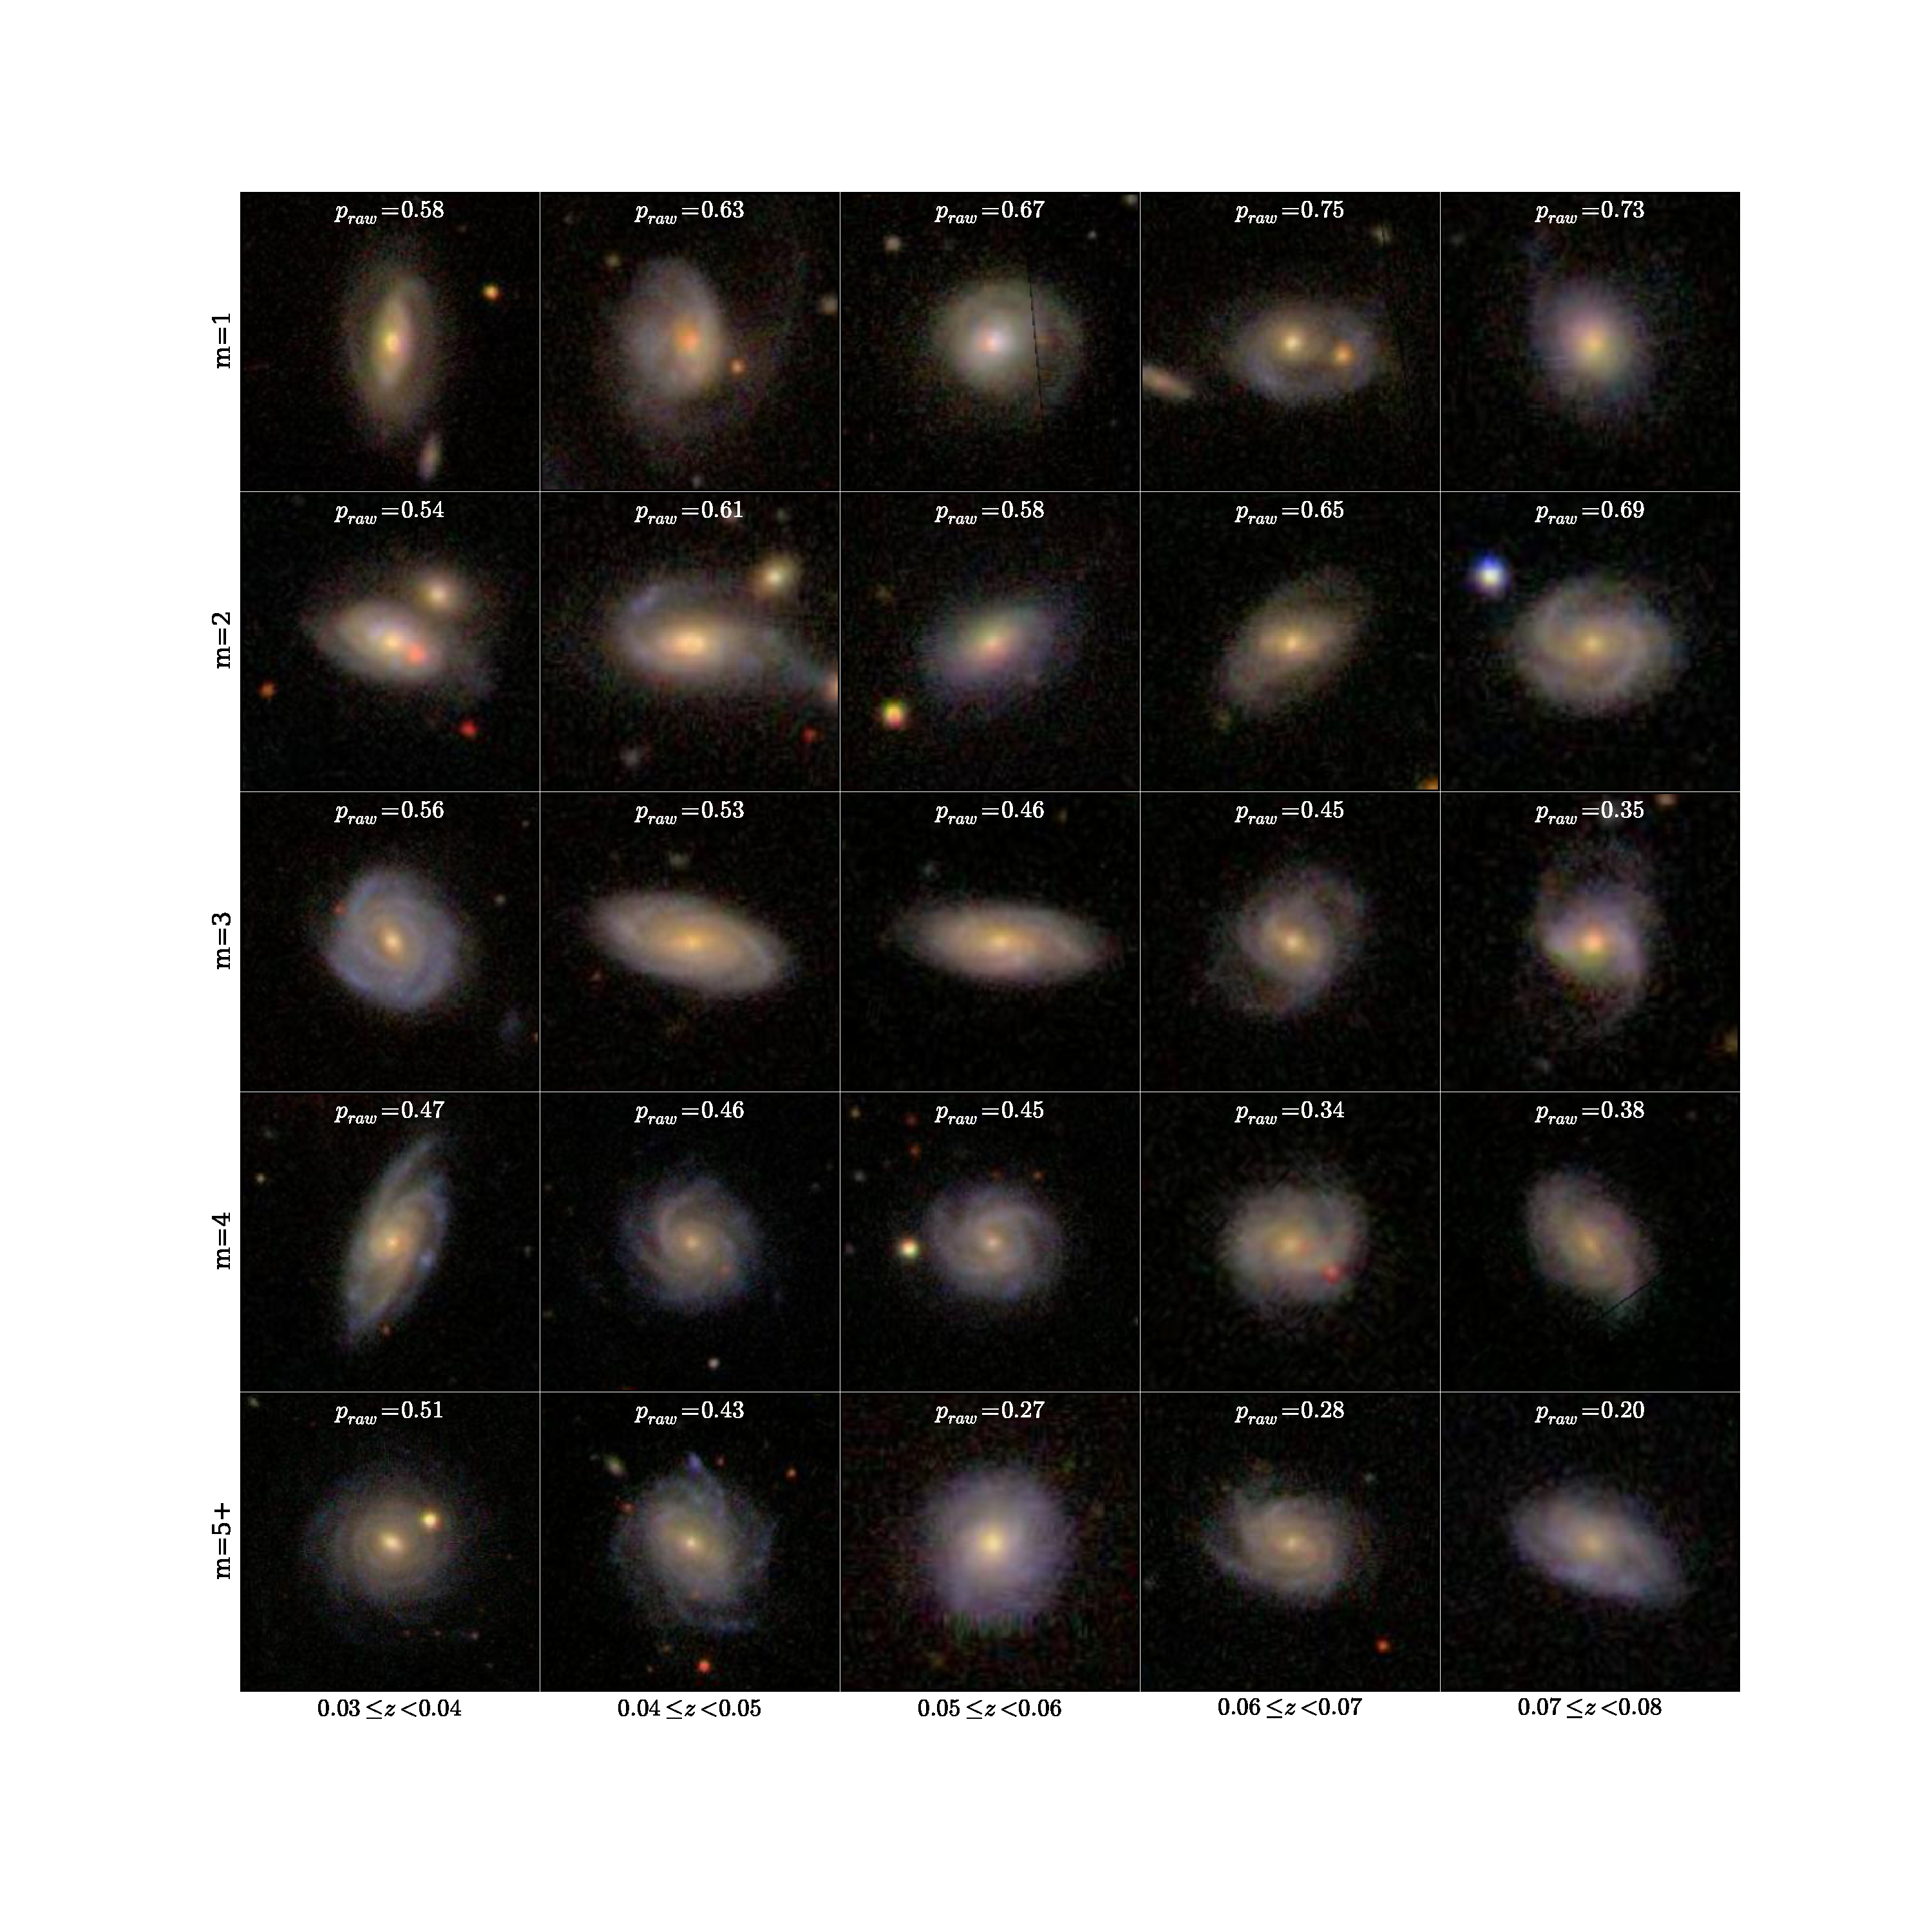
\includegraphics[width=1\textwidth]{Data_imgs/image_panel.pdf}
		
        \caption{Galaxies classified as 1,2,3,4 or more than 4 armed in different redshift ($z$) bins. Each of the galaxies is within a stellar mass range of $10.6 \leq \log(M/M_{\odot}) < 10.9$. The modal $p_m$ value (where $m$ is the spiral arm number) is within the range $0.5 \leq p_m < 0.6$.}
		
        \label{fig:image_panel}
        
\end{figure*}

\subsection{Comparison of relative sample sizes}

\rh{How big are each of the subsamples, when compared to the literature? This section may need a little more work than originally thought- a lot of the early stuff will deliberately select galaxies in different environments + w or w/o bars, so we may need to do something similar to check our fractions. Maybe use Yang+'s group catalogue, and the GZ bar fractions to define field galaxies and stuff like that to get an estimate of our completeness. This will also have to be compared to the original debiasing to show that we are doing 'better' I guess.}

\subsection{Stellar mass}
\label{sec:mass}

The distributions of stellar mass for each of the samples is shown in figure \ref{fig:mass_histogram}. From these plots, it is clear that there is no explicit dependence of arm number with stellar mass- each of the samples with different numbers of spiral arms spans the entire range of stellar mass from $10^{9} - 10^{11.5} M_{\odot}$. It must also be noted that the distributions in figure \ref{fig:mass_histogram} are of the \textit{luminosity limited sample}, and are therefore incomplete for low stellar mass objects (see section \ref{sec:VLS}). If we only consider the distributions above this stellar mass limit, then the galaxy samples look very different. Galaxies with more spiral arms generally seem to have higher stellar masses. 

This trend with stellar mass can be clearly seen when plotting the fraction of spiral galaxies with 1, 2, 3, 4 or more than 4 arms in bins of stellar mass, as shown in figure \ref{fig:mass_plot}. A clear trend is observed when looking at the highest stellar mass bins with $M_* \gtrsim 10^{11} M_{\odot}$. In the bins with lower stellar mass , the fraction of 2 and 5+ armed spiral galaxies remains consistent. However, a significant increase in galaxies with more than 4 spiral arms is observed in the most massive spiral galaxies with $M_* \gtrsim 10^{11} M_{\odot}$. In the bin of $M_* = 10^{11.97}M_{\odot}$, only $4 \pm 1 \%$ of galaxies are observed to have more than 4 spiral arms compared with $54 \pm 3 \%$ of the galaxies having 2 spiral arms. However, in the highest mass bin with $M_* = 10^{11.21}M_{\odot}$, a significant increase is seen in the fraction of 5+ armed spiral galaxies, with $15 \pm 2 \%$ of the galaxies have more than 4 spiral arms compared with $44 \pm 3 \%$ galaxies having 2 spiral arms. \rh{Numbers may change slightly with the new sample.}

\begin{figure}
		\centering
		
        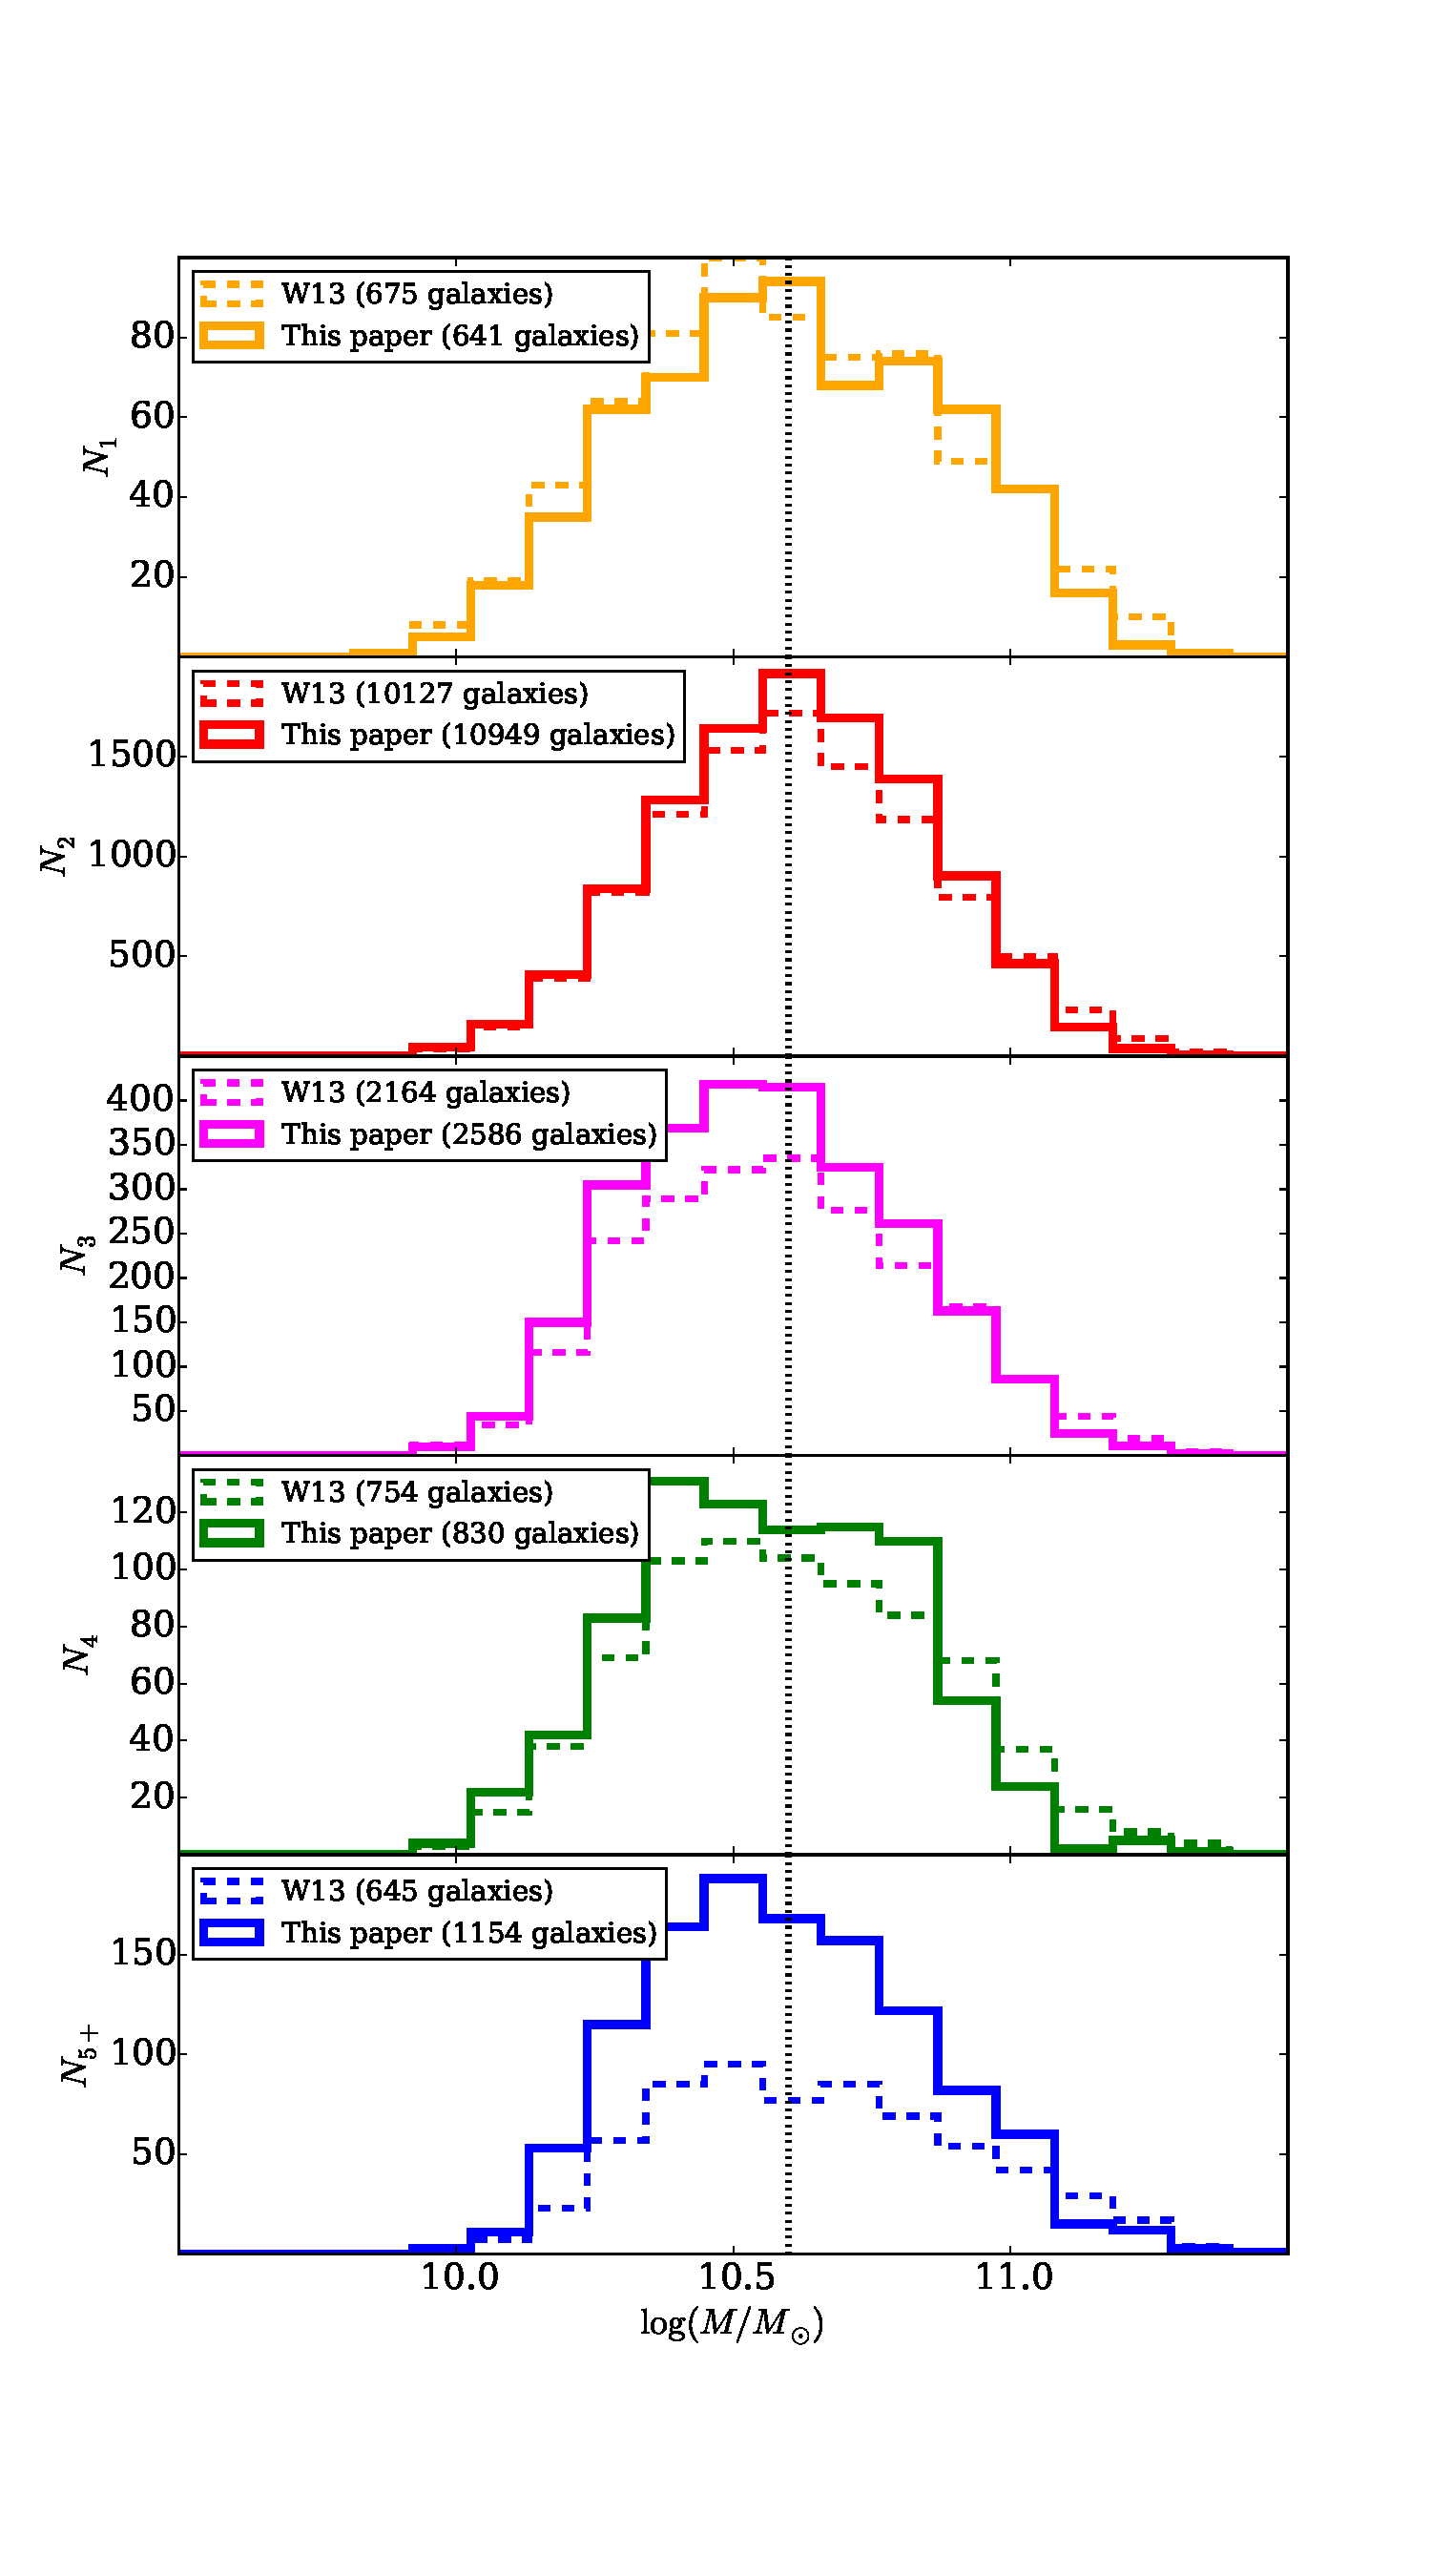
\includegraphics[width=0.5\textwidth]{Histograms/mass_histogram.pdf}
		
        \caption{Stellar mass distributions for the \textit{spiral sample}. the solid lines indicate the spiral sample defined using the debiasing described in section \ref{sec:new_method}, and the dashed line shows the same sample using the debiasing method in W13. The vertical dotted line shows the limit above which the data is stellar mass limited.}
		
        \label{fig:mass_histogram}
        
\end{figure}

\begin{figure}
		\centering
		
        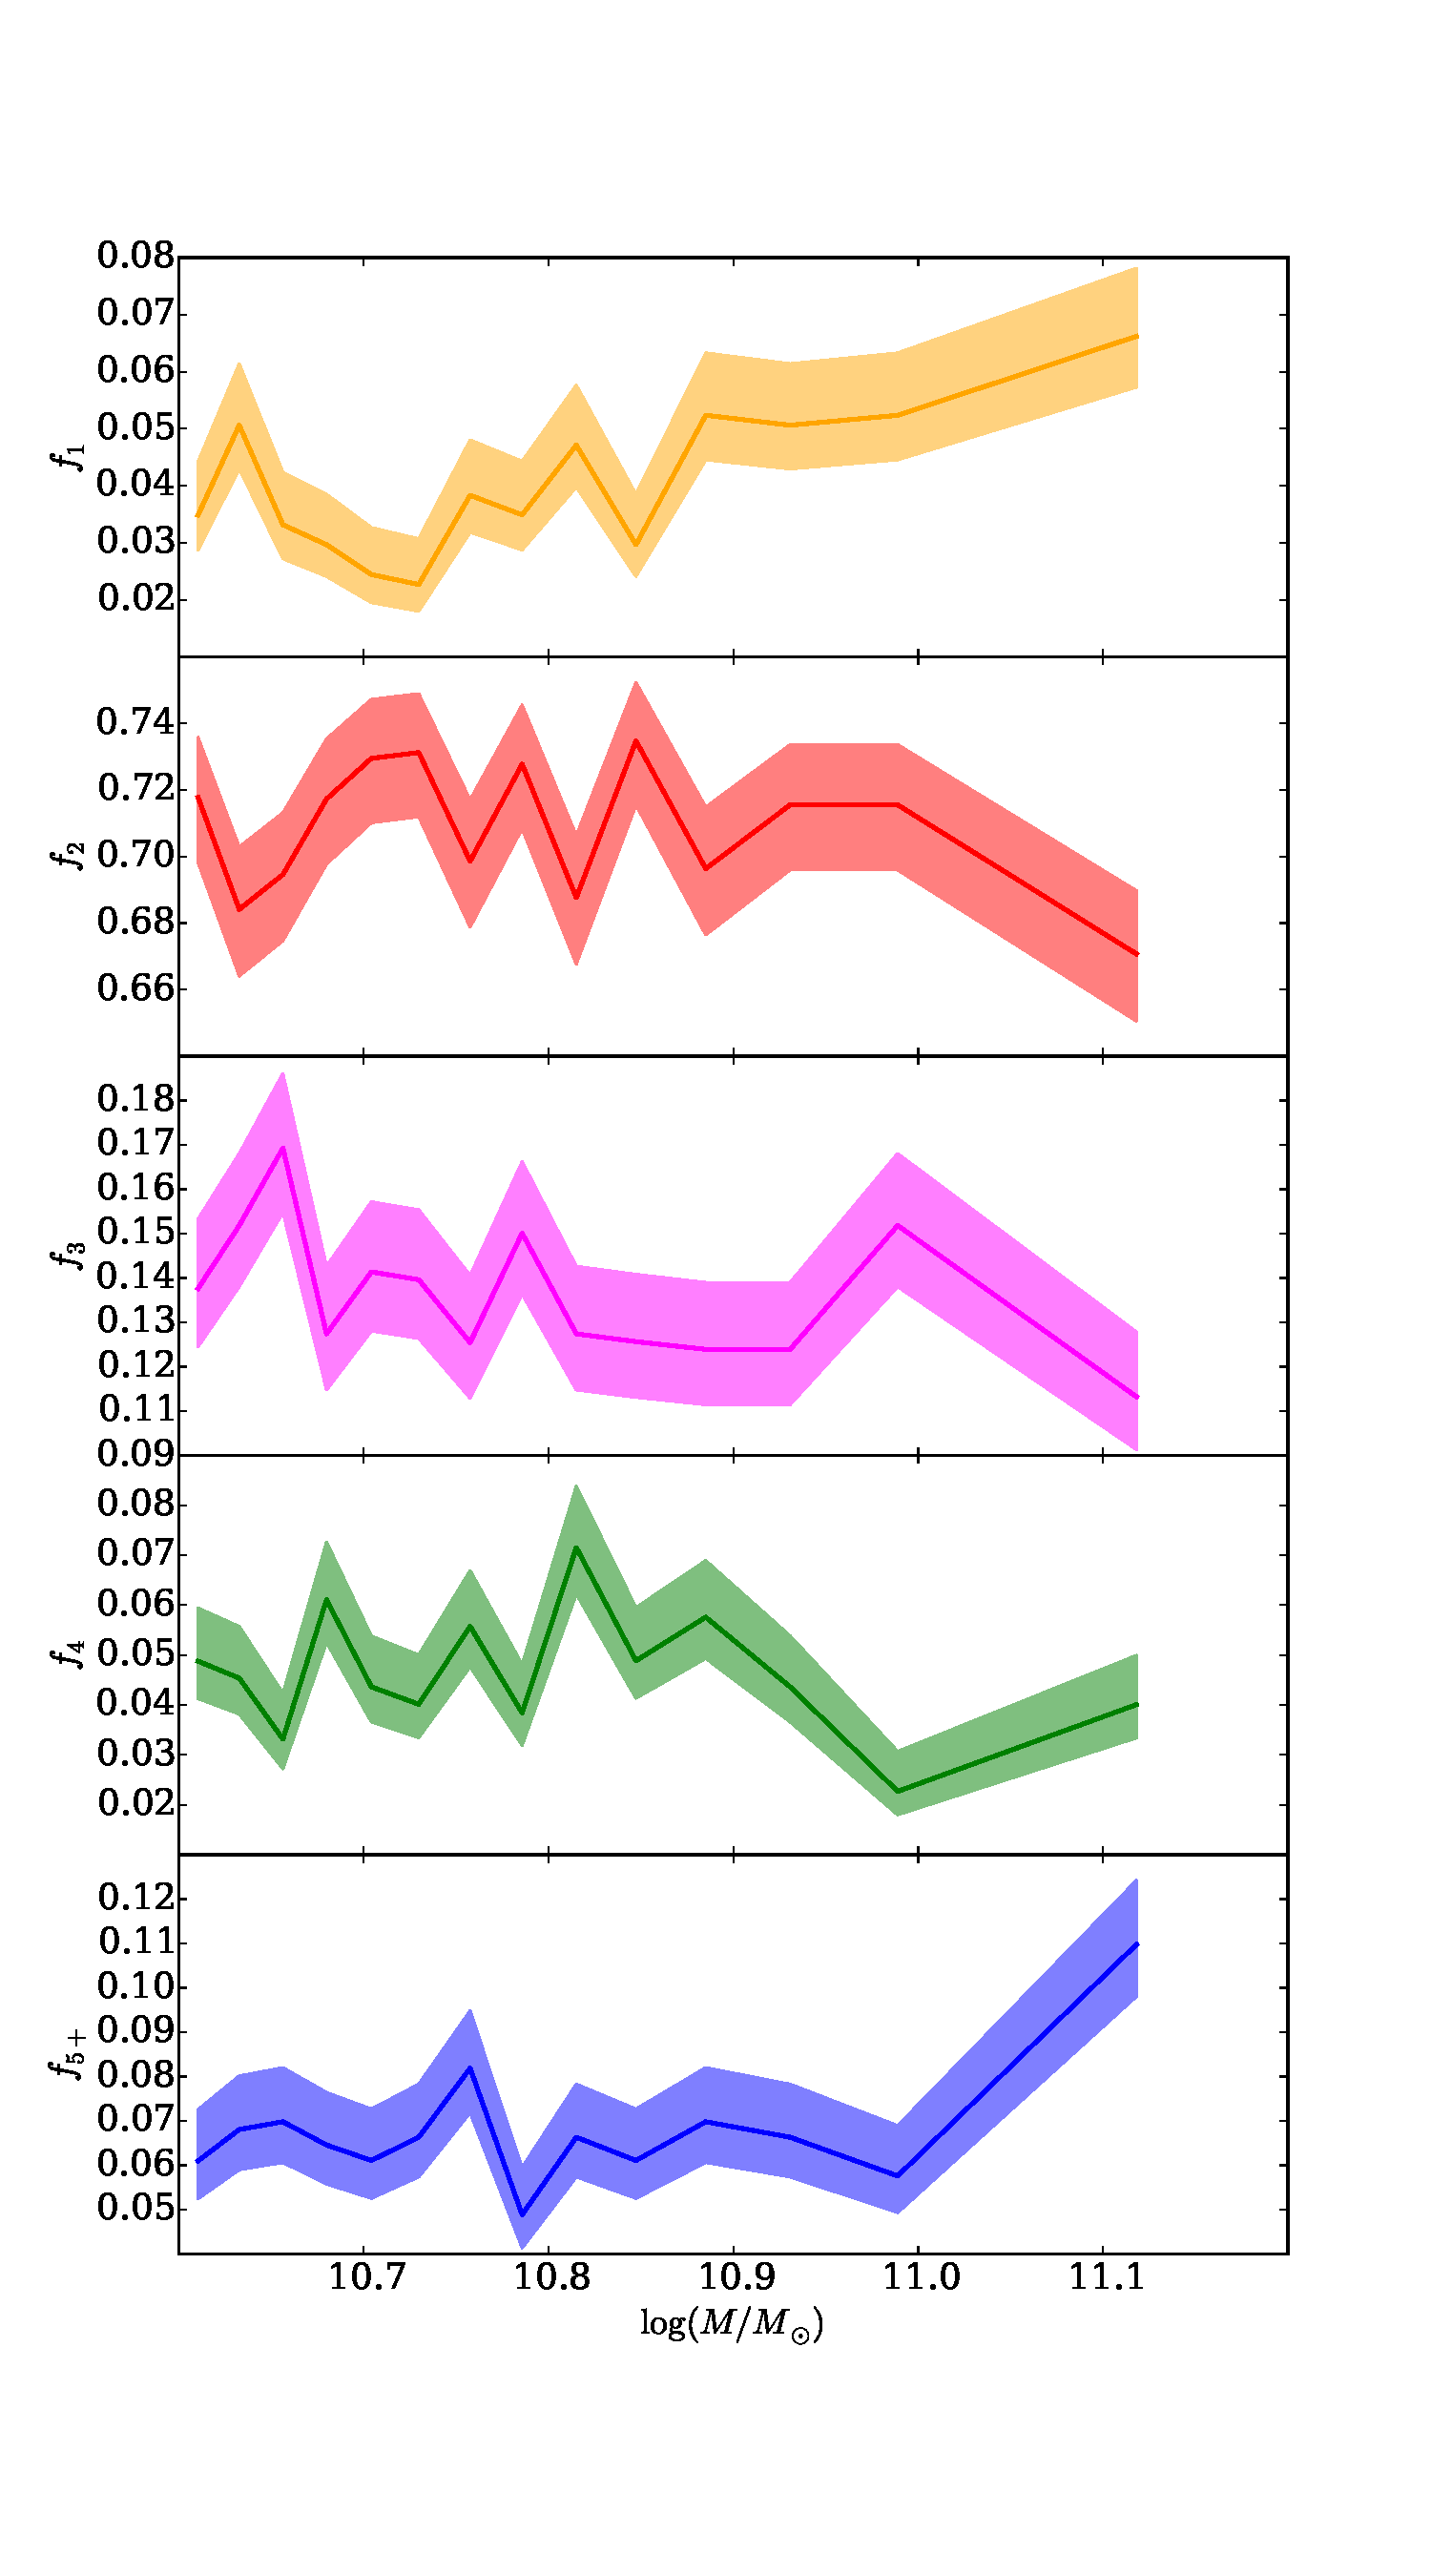
\includegraphics[width=0.5\textwidth]{Data_imgs/mass_plot.pdf}
		
        \caption{Fraction of galaxies with $m$ spiral arms for the stellar mass limited spiral sample, binned by stellar mass. The shaded region indicates the $\pm 1 \sigma$ error calculated using the method described in \protect\cite{Cameron_11}.}
		
        \label{fig:mass_plot}
        
\end{figure}

%------------------------------------------------------------------------------------

\subsection{Galaxy colours}

\begin{figure}
		\centering
		
        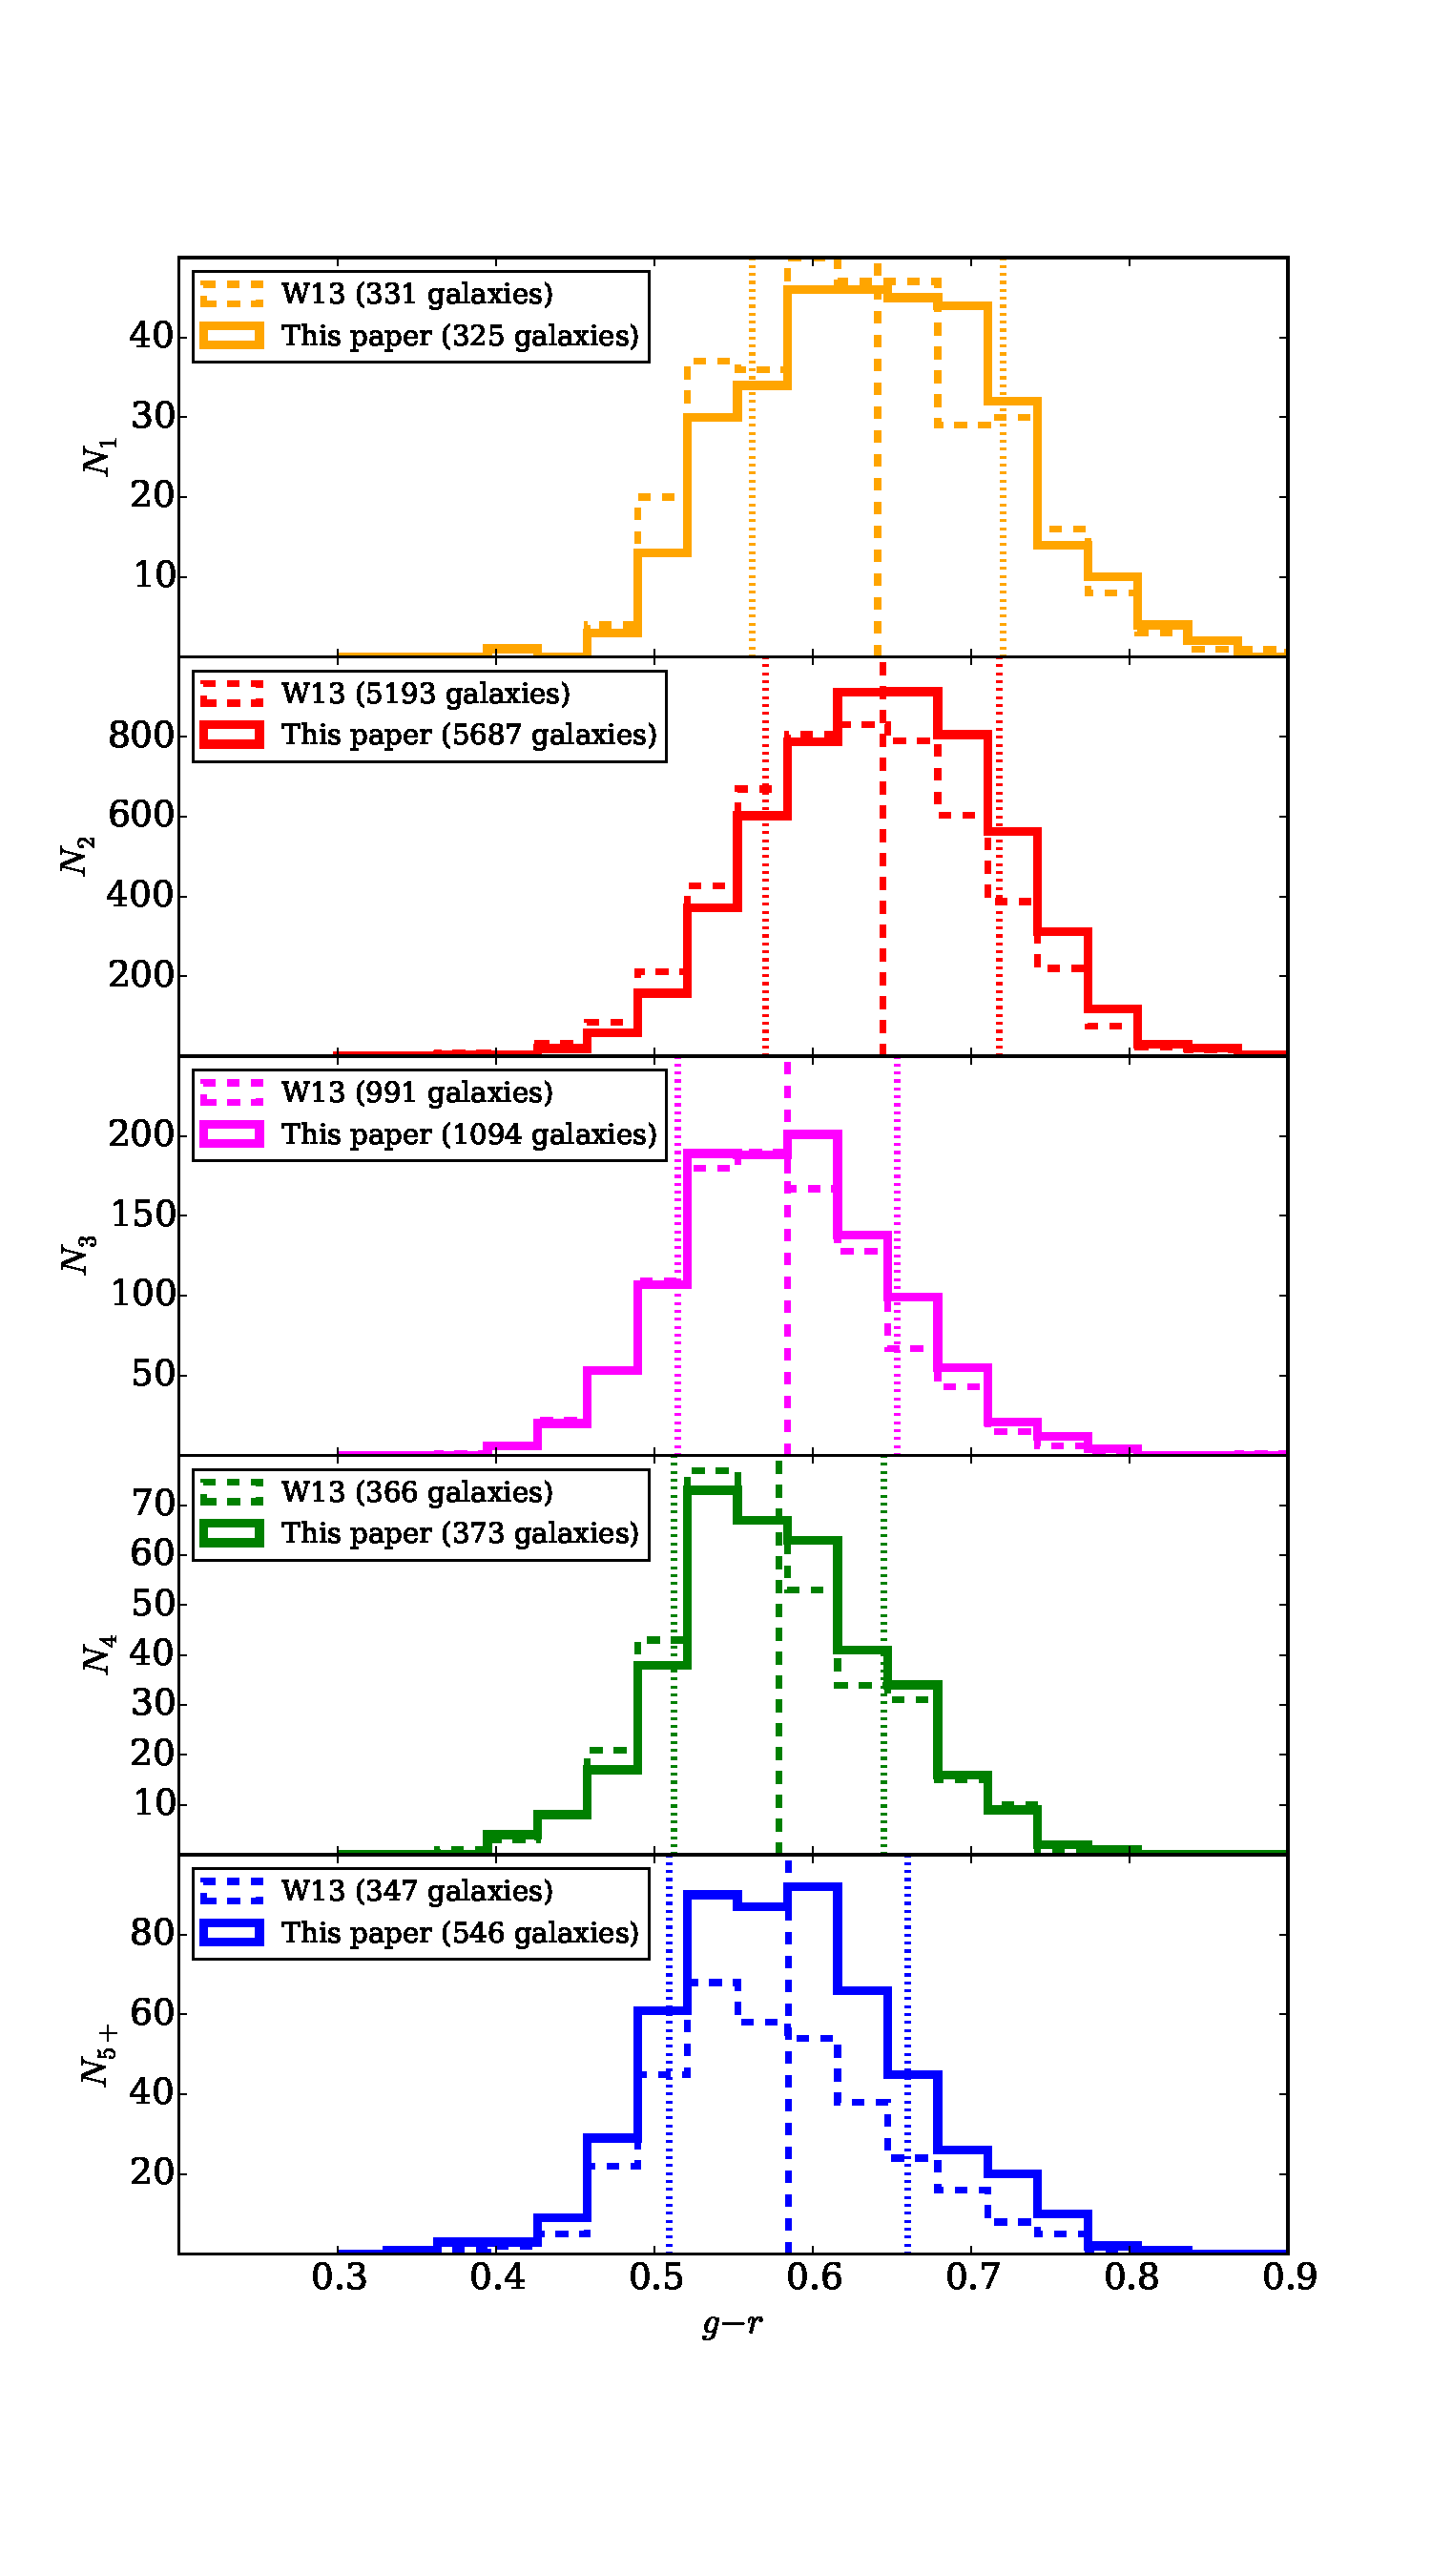
\includegraphics[width=0.5\textwidth]{Histograms/colour_histogram.pdf}
		
        \caption{Distribution of $g-r$ colours for the \textit{spiral sample} defined using our ddebiasing method (solid lines) and W13 (dashed lines). The vertical dashed lines show the mean $g-r$ colours and the dotted lines show $\pm1$ standard deviations.}
		
        \label{fig:colour_histogram}
        
\end{figure}

The galaxy sub-samples are also compared in terms of colour, in order to give an insight in to the star-formation properties of each of the samples. Bluer colours are generally associated with more recent star formation and therefore younger stellar populations. It is also well known that galaxy colour correlates with stellar mass, with more massive galaxies being redder in colour \citep{Baldry_06}. For this reason, the \textit{stellar mass limited sample} is used for this analysis to avoid any biases due to stellar mass differences. The distributions for each of the \textit{arm number samples} are shown in figure \ref{fig:colour_histogram}. There is a marked difference in the colours of the galaxies with many spiral arms, compared to the 2 armed galaxy population. The 2 armed spiral sample has a mean $g-r$ colour of 0.64 and a standard deviation of 0.07. Comparatively, the 4 and 5+ armed spirals both have a mean $g-r$ colour of 0.57 and a standard deviation of 0.07. For comparison, the standard deviation of the entire spiral sample is 0.08, so the associated shift colour shift between 2 armed and 4 or 5+ armed spirals corresponds to $\sim 1 \sigma$. This result is perhaps surprising, as the many-armed galaxies have greater stellar masses overall (section \ref{sec:mass}, which would normally mean that such galaxies are redder in colour \rh{cite}. The result therefore indicates that the stellar populations of many armed spiral galaxies are younger than the stellar populations in 2 armed spiral galaxies. 

\begin{figure}
		\centering
		
        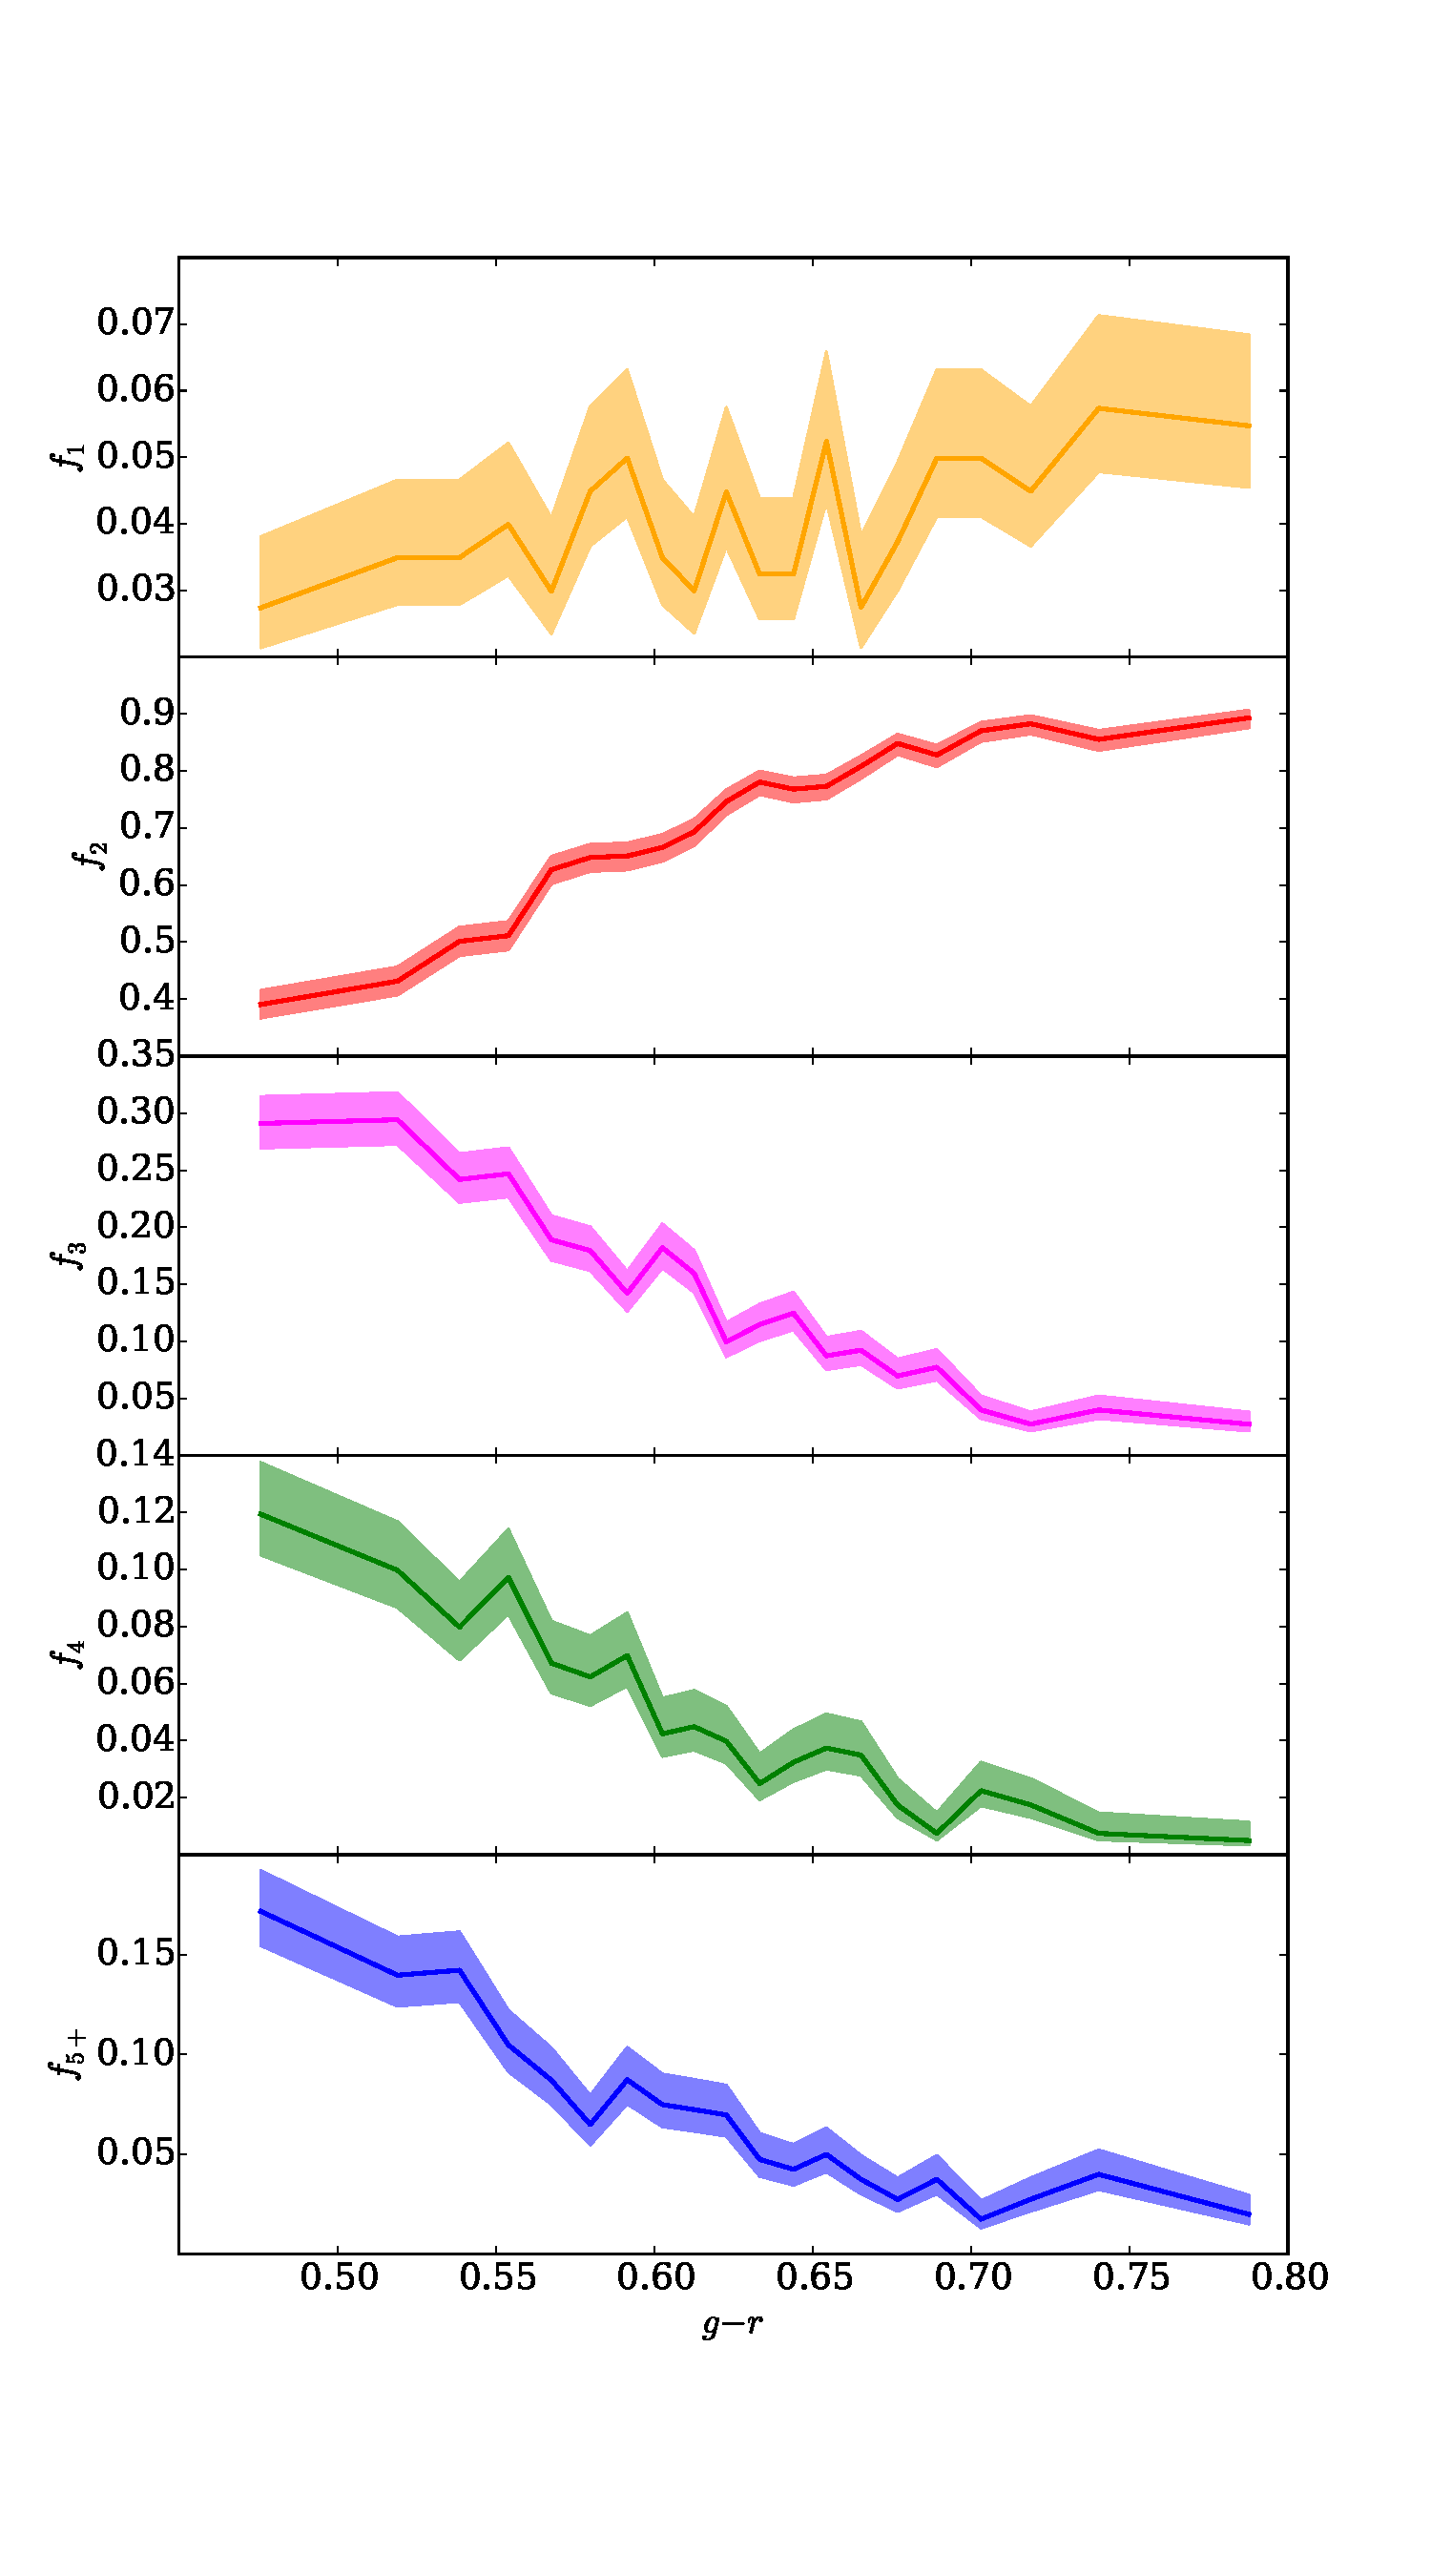
\includegraphics[width=0.5\textwidth]{Data_imgs/colour_plot.pdf}
		
        \caption{Fraction of galaxies with 1,2,3,4 or more than 4 arms binned by $g-r$ colour. The dotted line shows the mean fraction averaged over all of the bins for each of the samples, and the shaded region show the $1 \sigma$ errors.}
		
        \label{fig:colour_plot}
        
\end{figure}

The fraction of spirals with different numbers of spiral arms can also be compared by binning the data by colour, and the results are shown in figure \ref{fig:colour_plot}. The trends with colour seem to be much stronger than those observed with stellar mass in section \ref{sec:mass}, with all of the samples with the exception of the 1 armed galaxy sample showing a clear positive or negative correlation with colour. For the reddest population of galaxies, with $g-r=0.78$, the sample is dominated by grand design spiral structure, with $77 \pm 2 \%$ of the galaxies in that bin having 2 spiral arms. Conversely, in the bluest bin, with $g-r=0.47$, only $27 \pm 2 \%$ display 2 armed structure. The galaxies at the bluest end of the spectrum are dominated by galaxies with 3,4 or more than 4 spiral arms, with $57 \pm 3 \%$ of the galaxies in the bluest bin having 3,4 or more than 4 spiral arms compared to $6 \pm 1 \%$ in the bin containing the reddest spiral galaxies. 

%------------------------------------------------------------------------------------

\subsubsection{Star formation rates}
\label{sec:SFR}

The bluer colours of the many-armed spiral galaxies could be indicative of a higher star formation rate. We therefore plot the specific star formation rate distributions for each of spiral arm subsamples in figure \ref{fig:ssfr_histogram}. The distributions show that the bluer colours of the many armed spiral samples is not due to an enhanced star formation rate- the peaks of the distributions is not at a significantly higher value of sSFR. The main differences between the distributions are actually at the very highest and lowest ends of the sSFR scales. The 2 and more than 4 armed galaxies have an extended tail of low-sSFR galaxies that is not observed in the 3 and 4 armed galaxy distributions. The more than 4 armed distribution also shows that more than 4 armed galaxies do not have a significant fraction of galaxies with the very highest sSFRs, with the distribution seeming to have a maximimum value of $\sim 10^{-10} M_{\odot} yr^{-1}M_*^{-1}$. The only sample with a population of significantly enhanced sSFRs is the 1 armed galaxy sample. However, this result is unsurprising, as GZ classified 1 armed spiral galaxies have been associated with galaxy interactions in \citet{Casteels_13}, which itself is associated with enhanced star formation \rh{cite}.

\begin{figure}
		\centering
		
        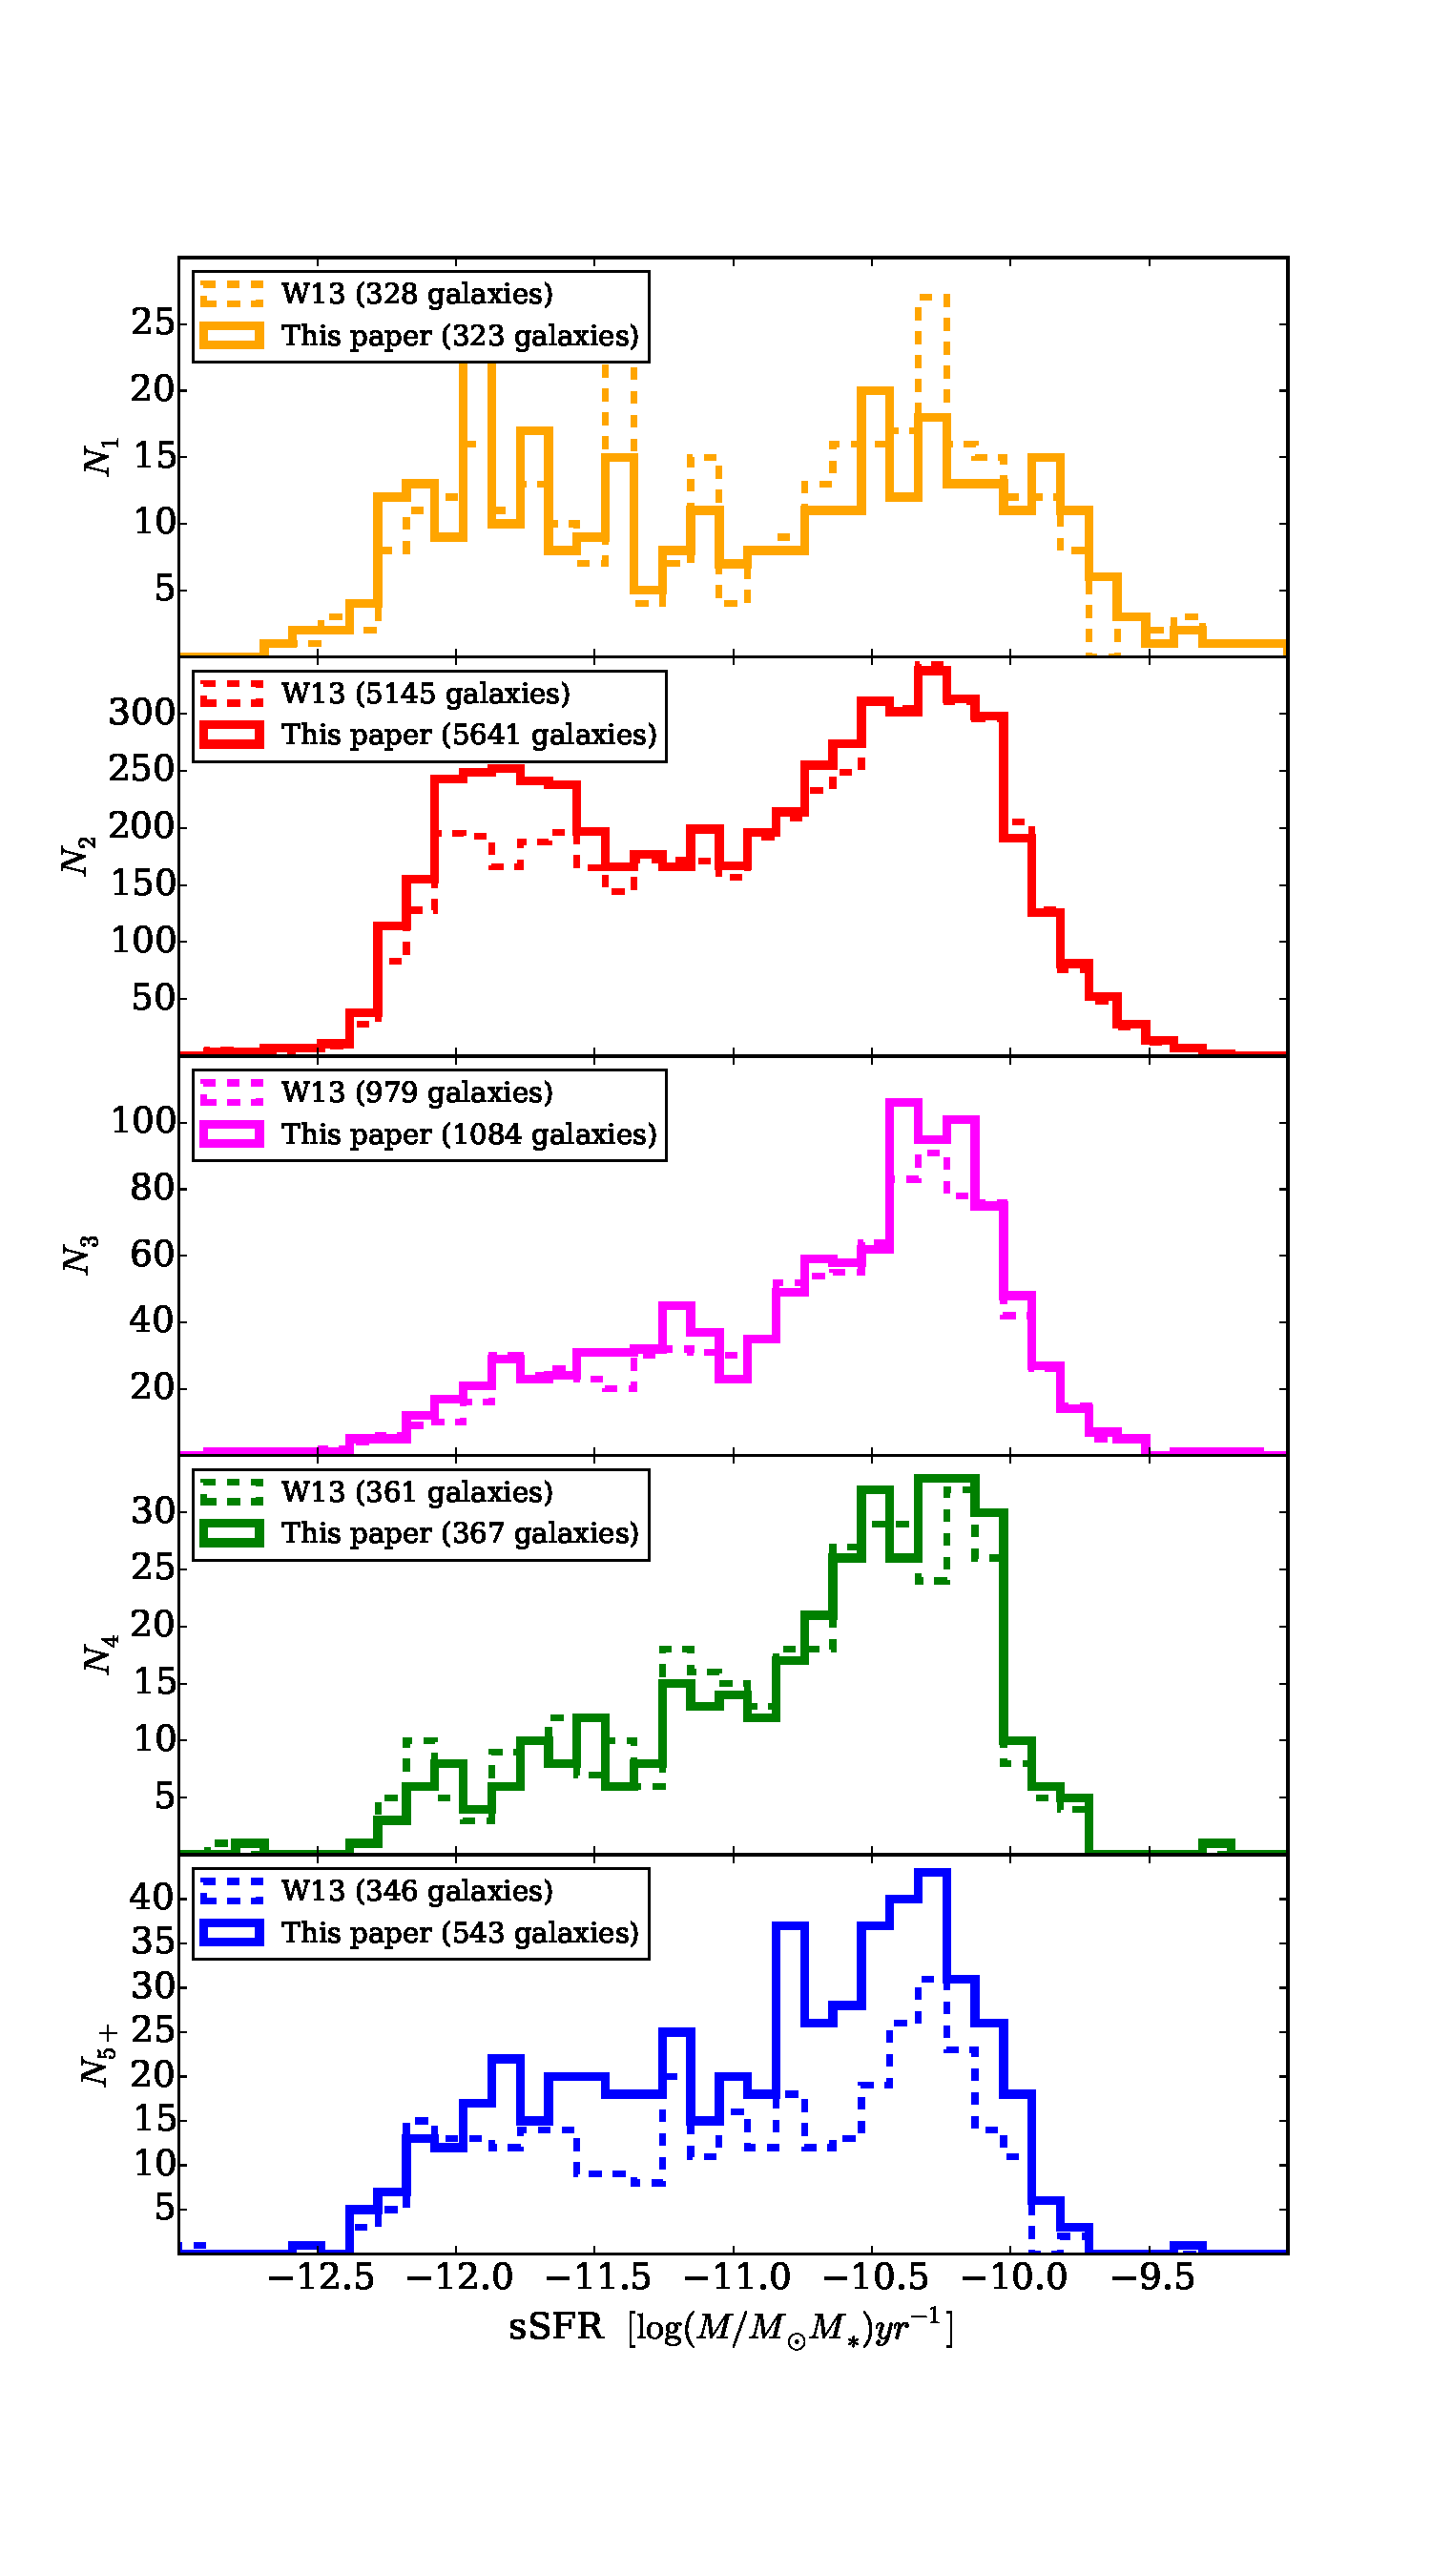
\includegraphics[width=0.5\textwidth]{Histograms/ssfr_histogram.pdf}
		
        \caption{Specific star formation rate histograms (sSFRs) for a \textit{spiral sample} from the \textit{stellar mass limited sample}. The solid lines show the sample from our debiasing procedure, and the dashed lines show a sample defined in the same way using the debiasing from W13.}
		
        \label{fig:ssfr_histogram}
        
\end{figure}

%------------------------------------------------------------------------------------
\subsubsection{Colour vs. stellar mass}
\label{sec:colour_mass}

Having demonstrated that the different galaxy populations have different stellar mass and colour properties, we now look in to these differences in more detail. The colour-mass contour is plotted for each of the subsamples in figure \ref{fig:cm1}, to check what the colour offset is with respect to stellar mass. The plots show that for a given stellar mass, the 3,4 and more than 4 armed galaxies are systematically bluer in the $g-r$ colour band. How much offset is observed for a given stellar mass is considered by fitting a best fit line to the data. The gradient of the line is set as constant using the entire \textit{stellar mass-limited spiral sample}. The calculated offsets indicate that for a given stellar mass, the 3 armed galaxy has a $g-r$ colour 0.06 lower than the 2 armed galaxy sample. The offsets in the 4 and 5+ armed samples are higher, with values of 0.07 and 0.08 respectively. \rh{Include some sigma values to attempt to quantify this result.}

\begin{figure}
		\centering
		
        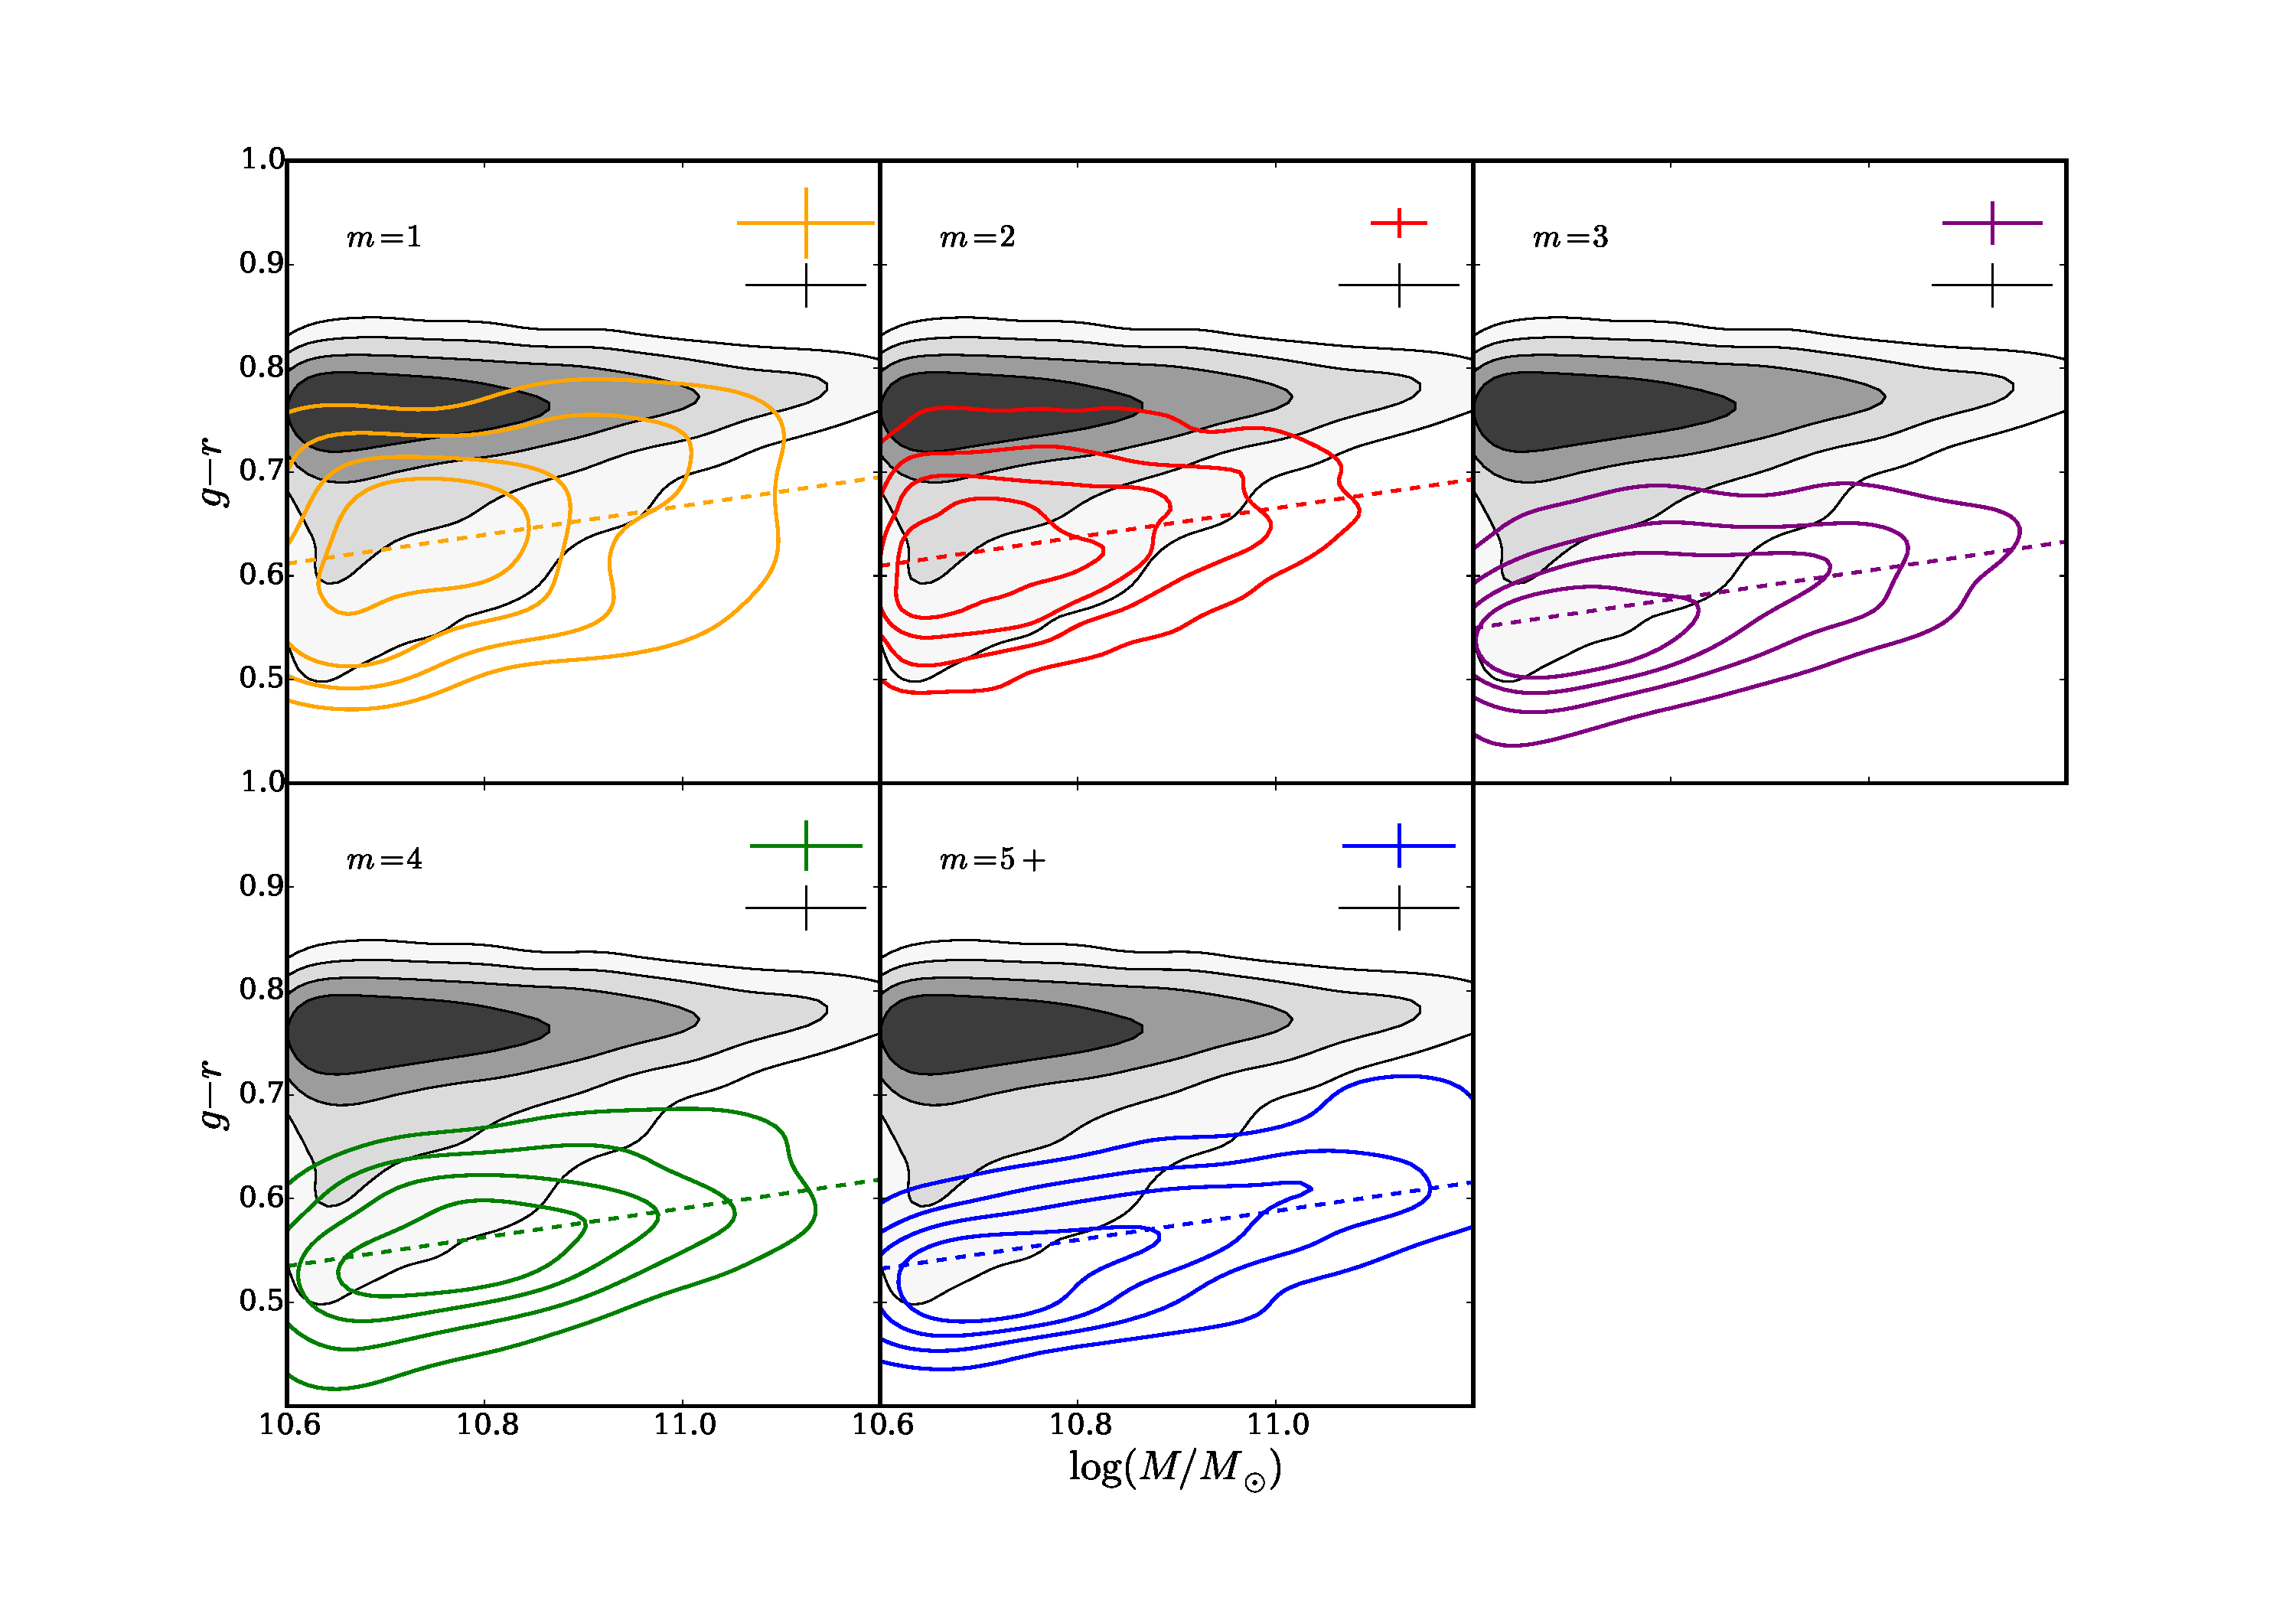
\includegraphics[width=0.5\textwidth]{Results_imgs/colour_mass_1.pdf}
		
        \caption{$g-r$ vs stellar mass for each of the \textit{stellar mass-limited arm number samples}. The grey filled contour indicates the full stellar mass limited sample. The contour lines extending outwards indicate the area enclosing 20,40,60 and 80\% of each sample. Each contour shows a kernel density estimate (KDE), optimised using 5-fold cross validation. The optimised bandwidths are indicated with the crosses in the top right-hand side of each figure. The dotted lines indicate the best fit line to the data, with a constant gradient of 0.14 set by the \textit{stellar mass-limited spiral sample}.}
		
        \label{fig:cm1}
        
\end{figure}
%------------------------------------------------------------------------------------
%%%%%%%%%%%%%%%%%%%%%%%%%%%%%%%%%%%%%%%%%%%%%%%%%%%%%%%%%%%%%%%%%%%%%%%%%%%%%%%%%%%%%
%------------------------------------------------------------------------------------
\section{Conclusions}
\label{sec:conclusions}

An examination of the properties of spiral galaxies with respect to their disk structure is presented using statistical morphological data from Galaxy Zoo. We show that employing a new debiasing procedure allows us to compare the properties of a spectroscopically complete sample of XX galaxies, of which XX can be classified as spirals and compared in terms of spiral arm number. Using this new debiasing method, clear differences in the overall properties of spiral galaxies are observed. By defining a stellar mass limited sample of spiral galaxies, it is seen that galaxies with greater numbers of spiral arms have higher stellar masses \rh{(Numbers?)}. A clear trend is also observed with respect to galaxy colour, with 4 and more than 4 armed spiral galaxies being much bluer in the $g-r$ colour band. The most stark contrast is observed when comparing the 2 armed spiral galaxy population with the more than 4 armed spiral galaxy population- we observe that for a given stellar mass, more than 4 armed spiral galaxies are $XX \pm XX$ bluer in $g-r$ than 2 armed spiral galaxies. However, there is no significant difference observed in the star formation rates of galaxies with different numbers of spiral arms. This suggests  that the $g-r$ colour differences are not attributable to more recent star formation in more than 4 armed spiral galaxies, and may therefore be due to 2 armed spiral galaxies having an older overall stellar population, or containing more dust.  

%------------------------------------------------------------------------------------
%%%%%%%%%%%%%%%%%%%%%%%%%%%%%%%%%%%%%%%%%%%%%%%%%%%%%%%%%%%%%%%%%%%%%%%%%%%%%%%%%%%%%
%------------------------------------------------------------------------------------

\section{Acknowledgements}

The data in this paper are the result of the efforts of the Galaxy Zoo 2 volunteers, without whom none of this work would be possible. Their efforts are individually acknowledged at authors.galaxyzoo.org.


\bibliographystyle{mn2e}
\bibliography{jun15}

\end{document}